% Options for packages loaded elsewhere
\PassOptionsToPackage{unicode}{hyperref}
\PassOptionsToPackage{hyphens}{url}
%
\documentclass[
]{book}
\usepackage{amsmath,amssymb}
\usepackage{iftex}
\ifPDFTeX
  \usepackage[T1]{fontenc}
  \usepackage[utf8]{inputenc}
  \usepackage{textcomp} % provide euro and other symbols
\else % if luatex or xetex
  \usepackage{unicode-math} % this also loads fontspec
  \defaultfontfeatures{Scale=MatchLowercase}
  \defaultfontfeatures[\rmfamily]{Ligatures=TeX,Scale=1}
\fi
\usepackage{lmodern}
\ifPDFTeX\else
  % xetex/luatex font selection
\fi
% Use upquote if available, for straight quotes in verbatim environments
\IfFileExists{upquote.sty}{\usepackage{upquote}}{}
\IfFileExists{microtype.sty}{% use microtype if available
  \usepackage[]{microtype}
  \UseMicrotypeSet[protrusion]{basicmath} % disable protrusion for tt fonts
}{}
\makeatletter
\@ifundefined{KOMAClassName}{% if non-KOMA class
  \IfFileExists{parskip.sty}{%
    \usepackage{parskip}
  }{% else
    \setlength{\parindent}{0pt}
    \setlength{\parskip}{6pt plus 2pt minus 1pt}}
}{% if KOMA class
  \KOMAoptions{parskip=half}}
\makeatother
\usepackage{xcolor}
\usepackage{longtable,booktabs,array}
\usepackage{calc} % for calculating minipage widths
% Correct order of tables after \paragraph or \subparagraph
\usepackage{etoolbox}
\makeatletter
\patchcmd\longtable{\par}{\if@noskipsec\mbox{}\fi\par}{}{}
\makeatother
% Allow footnotes in longtable head/foot
\IfFileExists{footnotehyper.sty}{\usepackage{footnotehyper}}{\usepackage{footnote}}
\makesavenoteenv{longtable}
\usepackage{graphicx}
\makeatletter
\def\maxwidth{\ifdim\Gin@nat@width>\linewidth\linewidth\else\Gin@nat@width\fi}
\def\maxheight{\ifdim\Gin@nat@height>\textheight\textheight\else\Gin@nat@height\fi}
\makeatother
% Scale images if necessary, so that they will not overflow the page
% margins by default, and it is still possible to overwrite the defaults
% using explicit options in \includegraphics[width, height, ...]{}
\setkeys{Gin}{width=\maxwidth,height=\maxheight,keepaspectratio}
% Set default figure placement to htbp
\makeatletter
\def\fps@figure{htbp}
\makeatother
\setlength{\emergencystretch}{3em} % prevent overfull lines
\providecommand{\tightlist}{%
  \setlength{\itemsep}{0pt}\setlength{\parskip}{0pt}}
\setcounter{secnumdepth}{5}
\usepackage{booktabs}
\ifLuaTeX
  \usepackage{selnolig}  % disable illegal ligatures
\fi
\usepackage[]{natbib}
\bibliographystyle{plainnat}
\usepackage{bookmark}
\IfFileExists{xurl.sty}{\usepackage{xurl}}{} % add URL line breaks if available
\urlstyle{same}
\hypersetup{
  pdftitle={Baby Rudin},
  pdfauthor={Ashan Jayamal},
  hidelinks,
  pdfcreator={LaTeX via pandoc}}

\title{Baby Rudin}
\author{Ashan Jayamal}
\date{2024-09-21}

\usepackage{amsthm}
\newtheorem{theorem}{Theorem}[chapter]
\newtheorem{lemma}{Lemma}[chapter]
\newtheorem{corollary}{Corollary}[chapter]
\newtheorem{proposition}{Proposition}[chapter]
\newtheorem{conjecture}{Conjecture}[chapter]
\theoremstyle{definition}
\newtheorem{definition}{Definition}[chapter]
\theoremstyle{definition}
\newtheorem{example}{Example}[chapter]
\theoremstyle{definition}
\newtheorem{exercise}{Exercise}[chapter]
\theoremstyle{definition}
\newtheorem{hypothesis}{Hypothesis}[chapter]
\theoremstyle{remark}
\newtheorem*{remark}{Remark}
\newtheorem*{solution}{Solution}
\begin{document}
\maketitle

{
\setcounter{tocdepth}{1}
\tableofcontents
}
\chapter{The Real and Complex Number Systems}\label{the-real-and-complex-number-systems}

\section{Exercise}\label{exercise}

\begin{exercise}
\protect\hypertarget{exr:unnamed-chunk-1}{}\label{exr:unnamed-chunk-1}If \(r\) is rational \(r\neq 0\) and x is irrational, prove that \(r + x\) and \(rx\) are irrational.
\end{exercise}

Suppose that \(0 \neq r \in \mathbb{Q}\) and \(x\in \mathbb{R}\setminus \mathbb{Q}\)

\begin{itemize}
\item
  \textbf{Claim 1}: \(r+x\) is irrational.\\
  Assume the contray that \(r+x\in \mathbb{Q}\). Since, \(\mathbb{Q}\) is field,
  \[x=(r+x)-r\in \mathbb{Q}\]. This is a contradiction. Thus, \(r+x\) is contradiction.
\item
  \textbf{Claim 2}: \(rx\) is irrational.\\
  Assume the contray that \(rx\in \mathbb{Q}\). Since, \(\mathbb{Q}\) is field,
  \[\left(\frac{1}{x}\right)rx=\left(\frac{1}{x}\right)xr=\left(\frac{1}{x}x\right)r=x\in \mathbb{Q}\]. This is a contradiction. Thus, \(r+x\) is contradiction.
\end{itemize}

\begin{exercise}[1:R2]
\protect\hypertarget{exr:unnamed-chunk-2}{}\label{exr:unnamed-chunk-2}Prove that there is no rational number whose square is 12.
\end{exercise}

\begin{proof}
First observe that
\[\sqrt{12}=\sqrt{4\cdot 3}=2\sqrt{3}\]

\textbf{Claim 1} : \(\forall n\in \mathbb{N}3|n^2 \implies 3|n\).\\
Let \(n\in \mathbb{N}\). Suppose that \(3|n^2\) We know that \(3\) is prime. Then by number theory resuts we can get \(3|n\) or \(3|n\).
We are done.

\textbf{Cliam 2}: \(\sqrt{3}\) is irrartional.\\
We use inderect proof. Assume contary, \(\sqrt{3}\) is rational. In other words,
\[\sqrt{3}=\frac{p}{q}\text{  for some } q\in \mathbb{Z} , q\neq 0\text{ and } p,q \text{ have no comman factors.}\]
Thus,\[3q^2=p^2\]
Then, by above claim we can get that \(3|p\). Thus, there exists \(k \in \mathbb{Z}\) such that \(3k=p\).
Thus,
\[
\begin{aligned}
3q^2 &=p^2\\
3q^2 &= (3k)^2\\
3q^2 &= 9k^2\\
q^2  &= 3k^2
\end{aligned}
\]
So, both \(p\) and \(q\) have comman factor 3.This contract our assumption. Thefore, \(\sqrt(3)\) is irrational. So we are done proof of claim 2.

Since, \(\sqrt{3}\) is not a rational number. Thus \(\sqrt{3}\) is irrational number.
\end{proof}

\begin{exercise}
\protect\hypertarget{exr:unnamed-chunk-4}{}\label{exr:unnamed-chunk-4}Prove Proposition 1.15.
\end{exercise}

\begin{exercise}
\protect\hypertarget{exr:unnamed-chunk-5}{}\label{exr:unnamed-chunk-5}Let \(E\) be a nonempty subset of an ordered set. Suppose \(\alpha\) is a lower bound of \(E\) and \(\beta\) is an upper bound of \(E\). Prove that \(\alpha \leq \beta\).
\end{exercise}

\section{Written Answers}\label{written-answers}

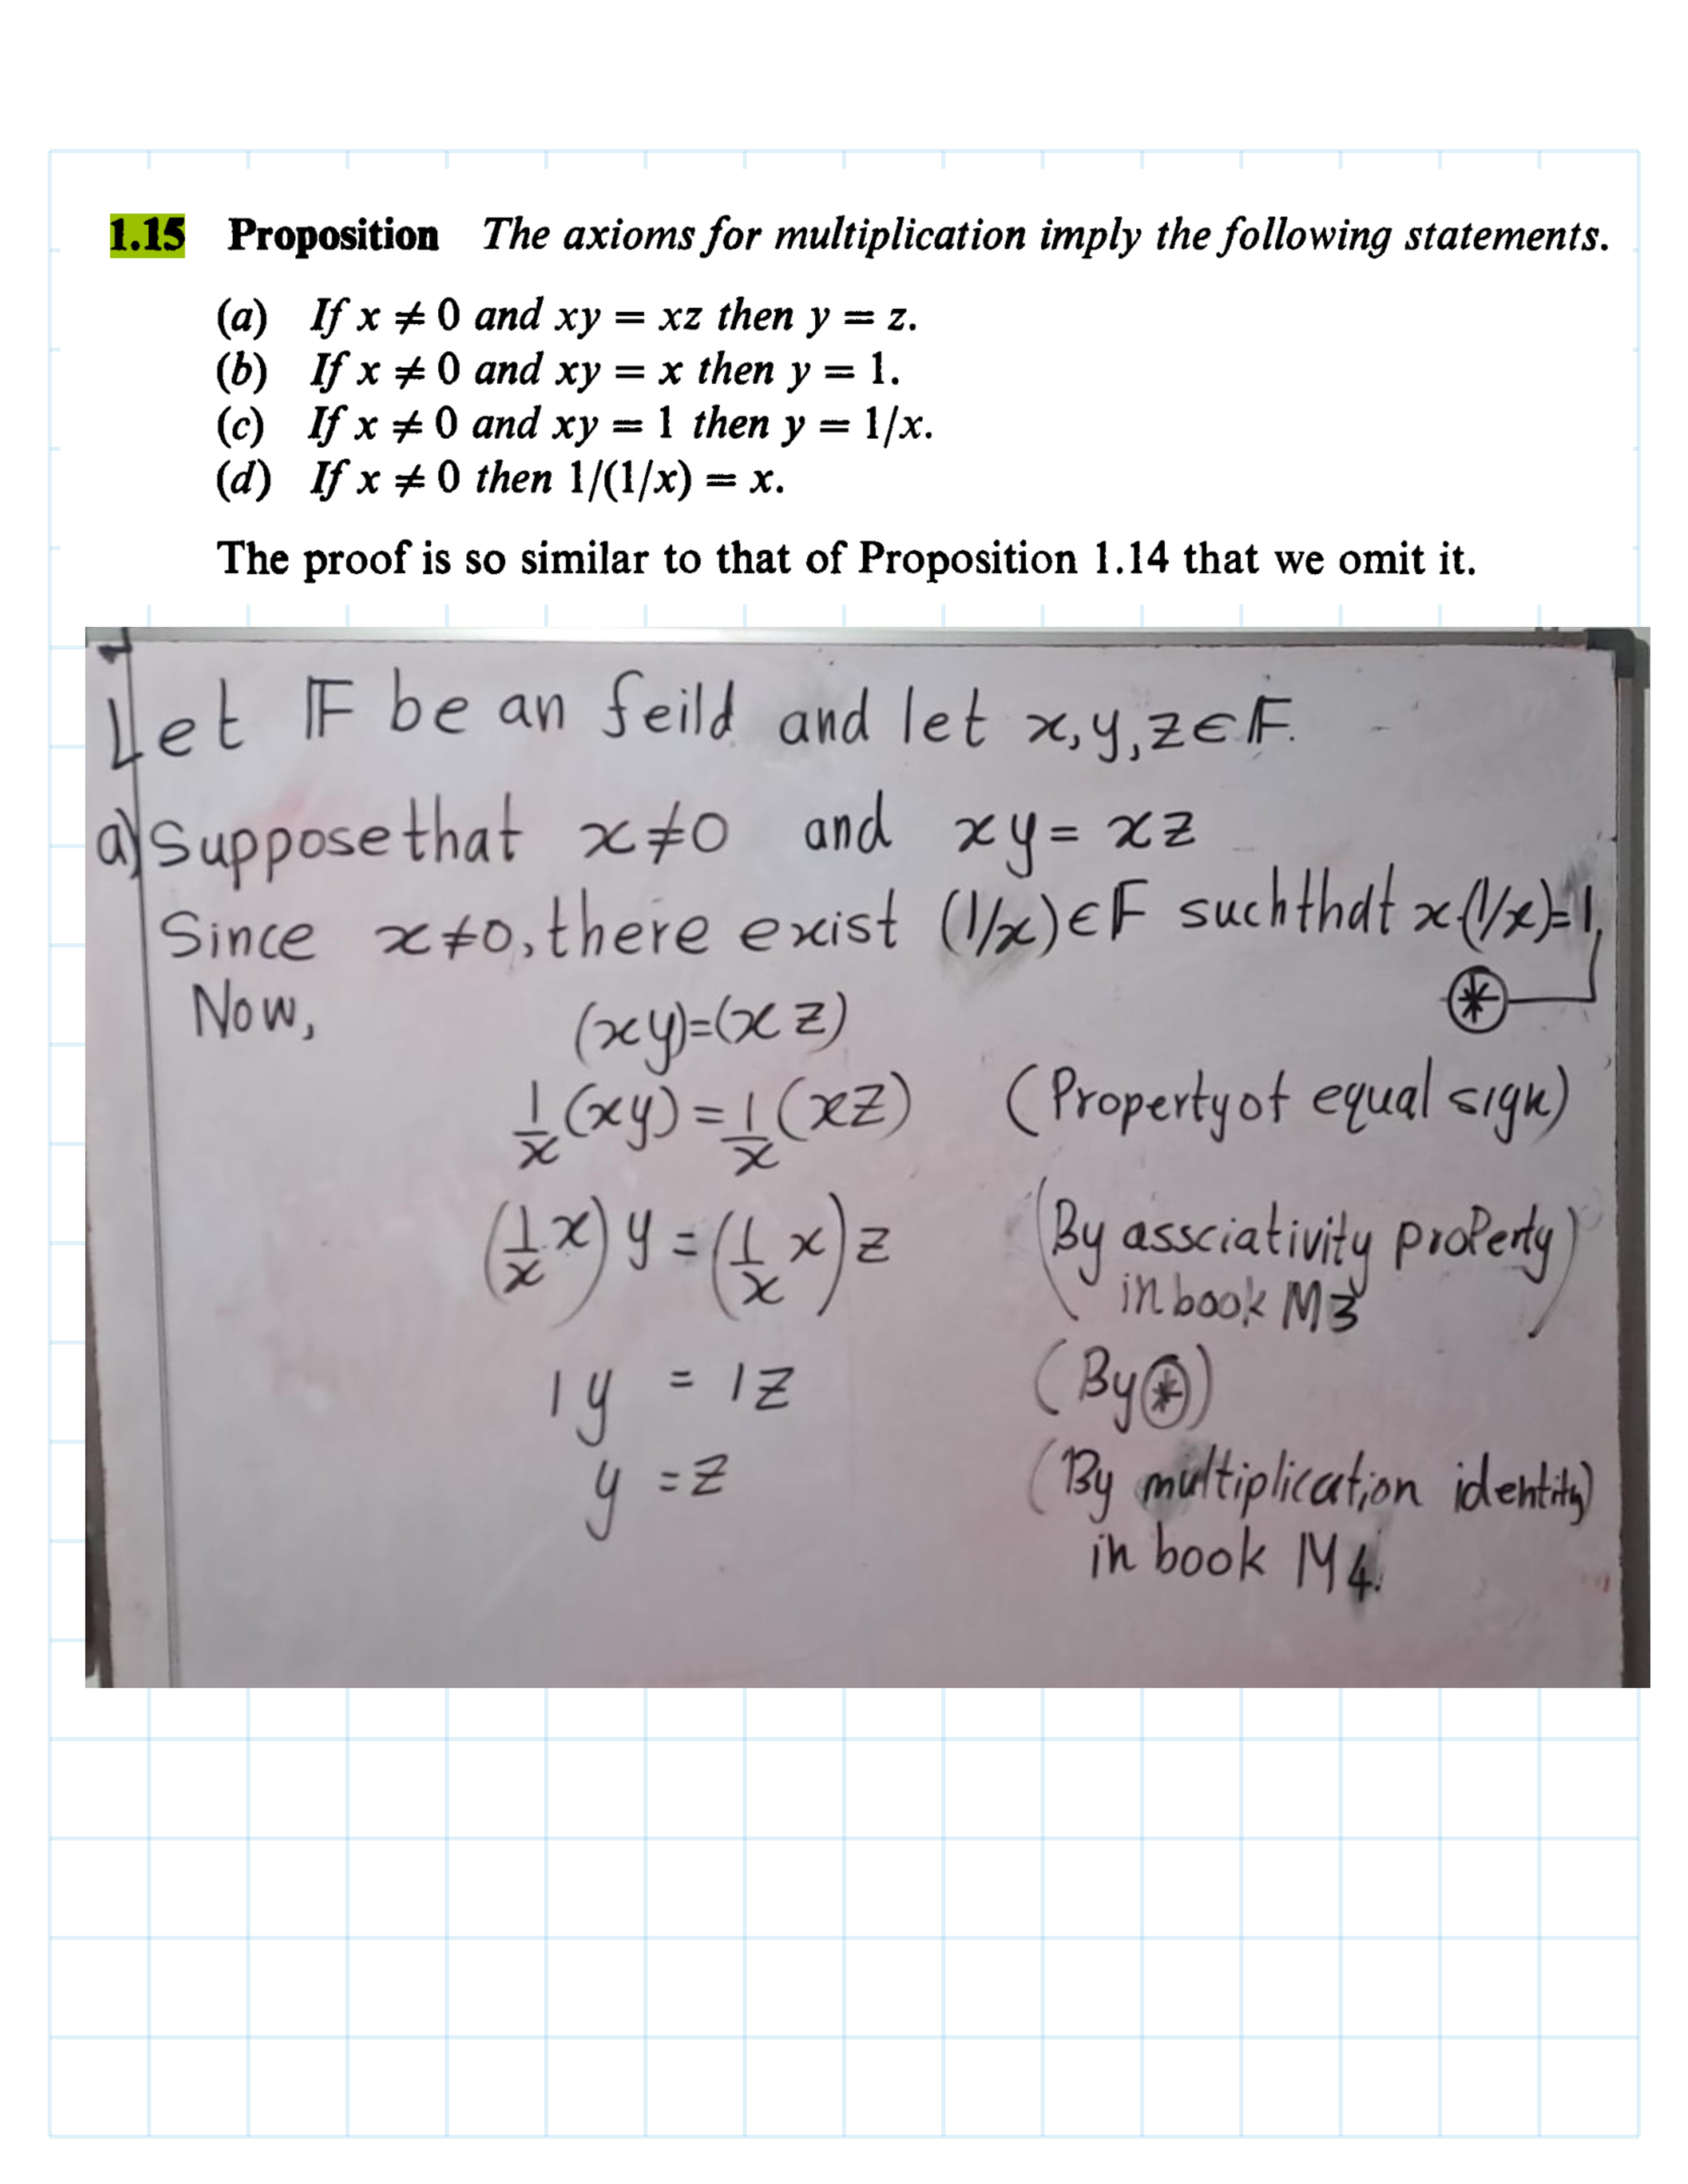
\includegraphics{Figures/Ex-1/Rudin-Ex (1).png}
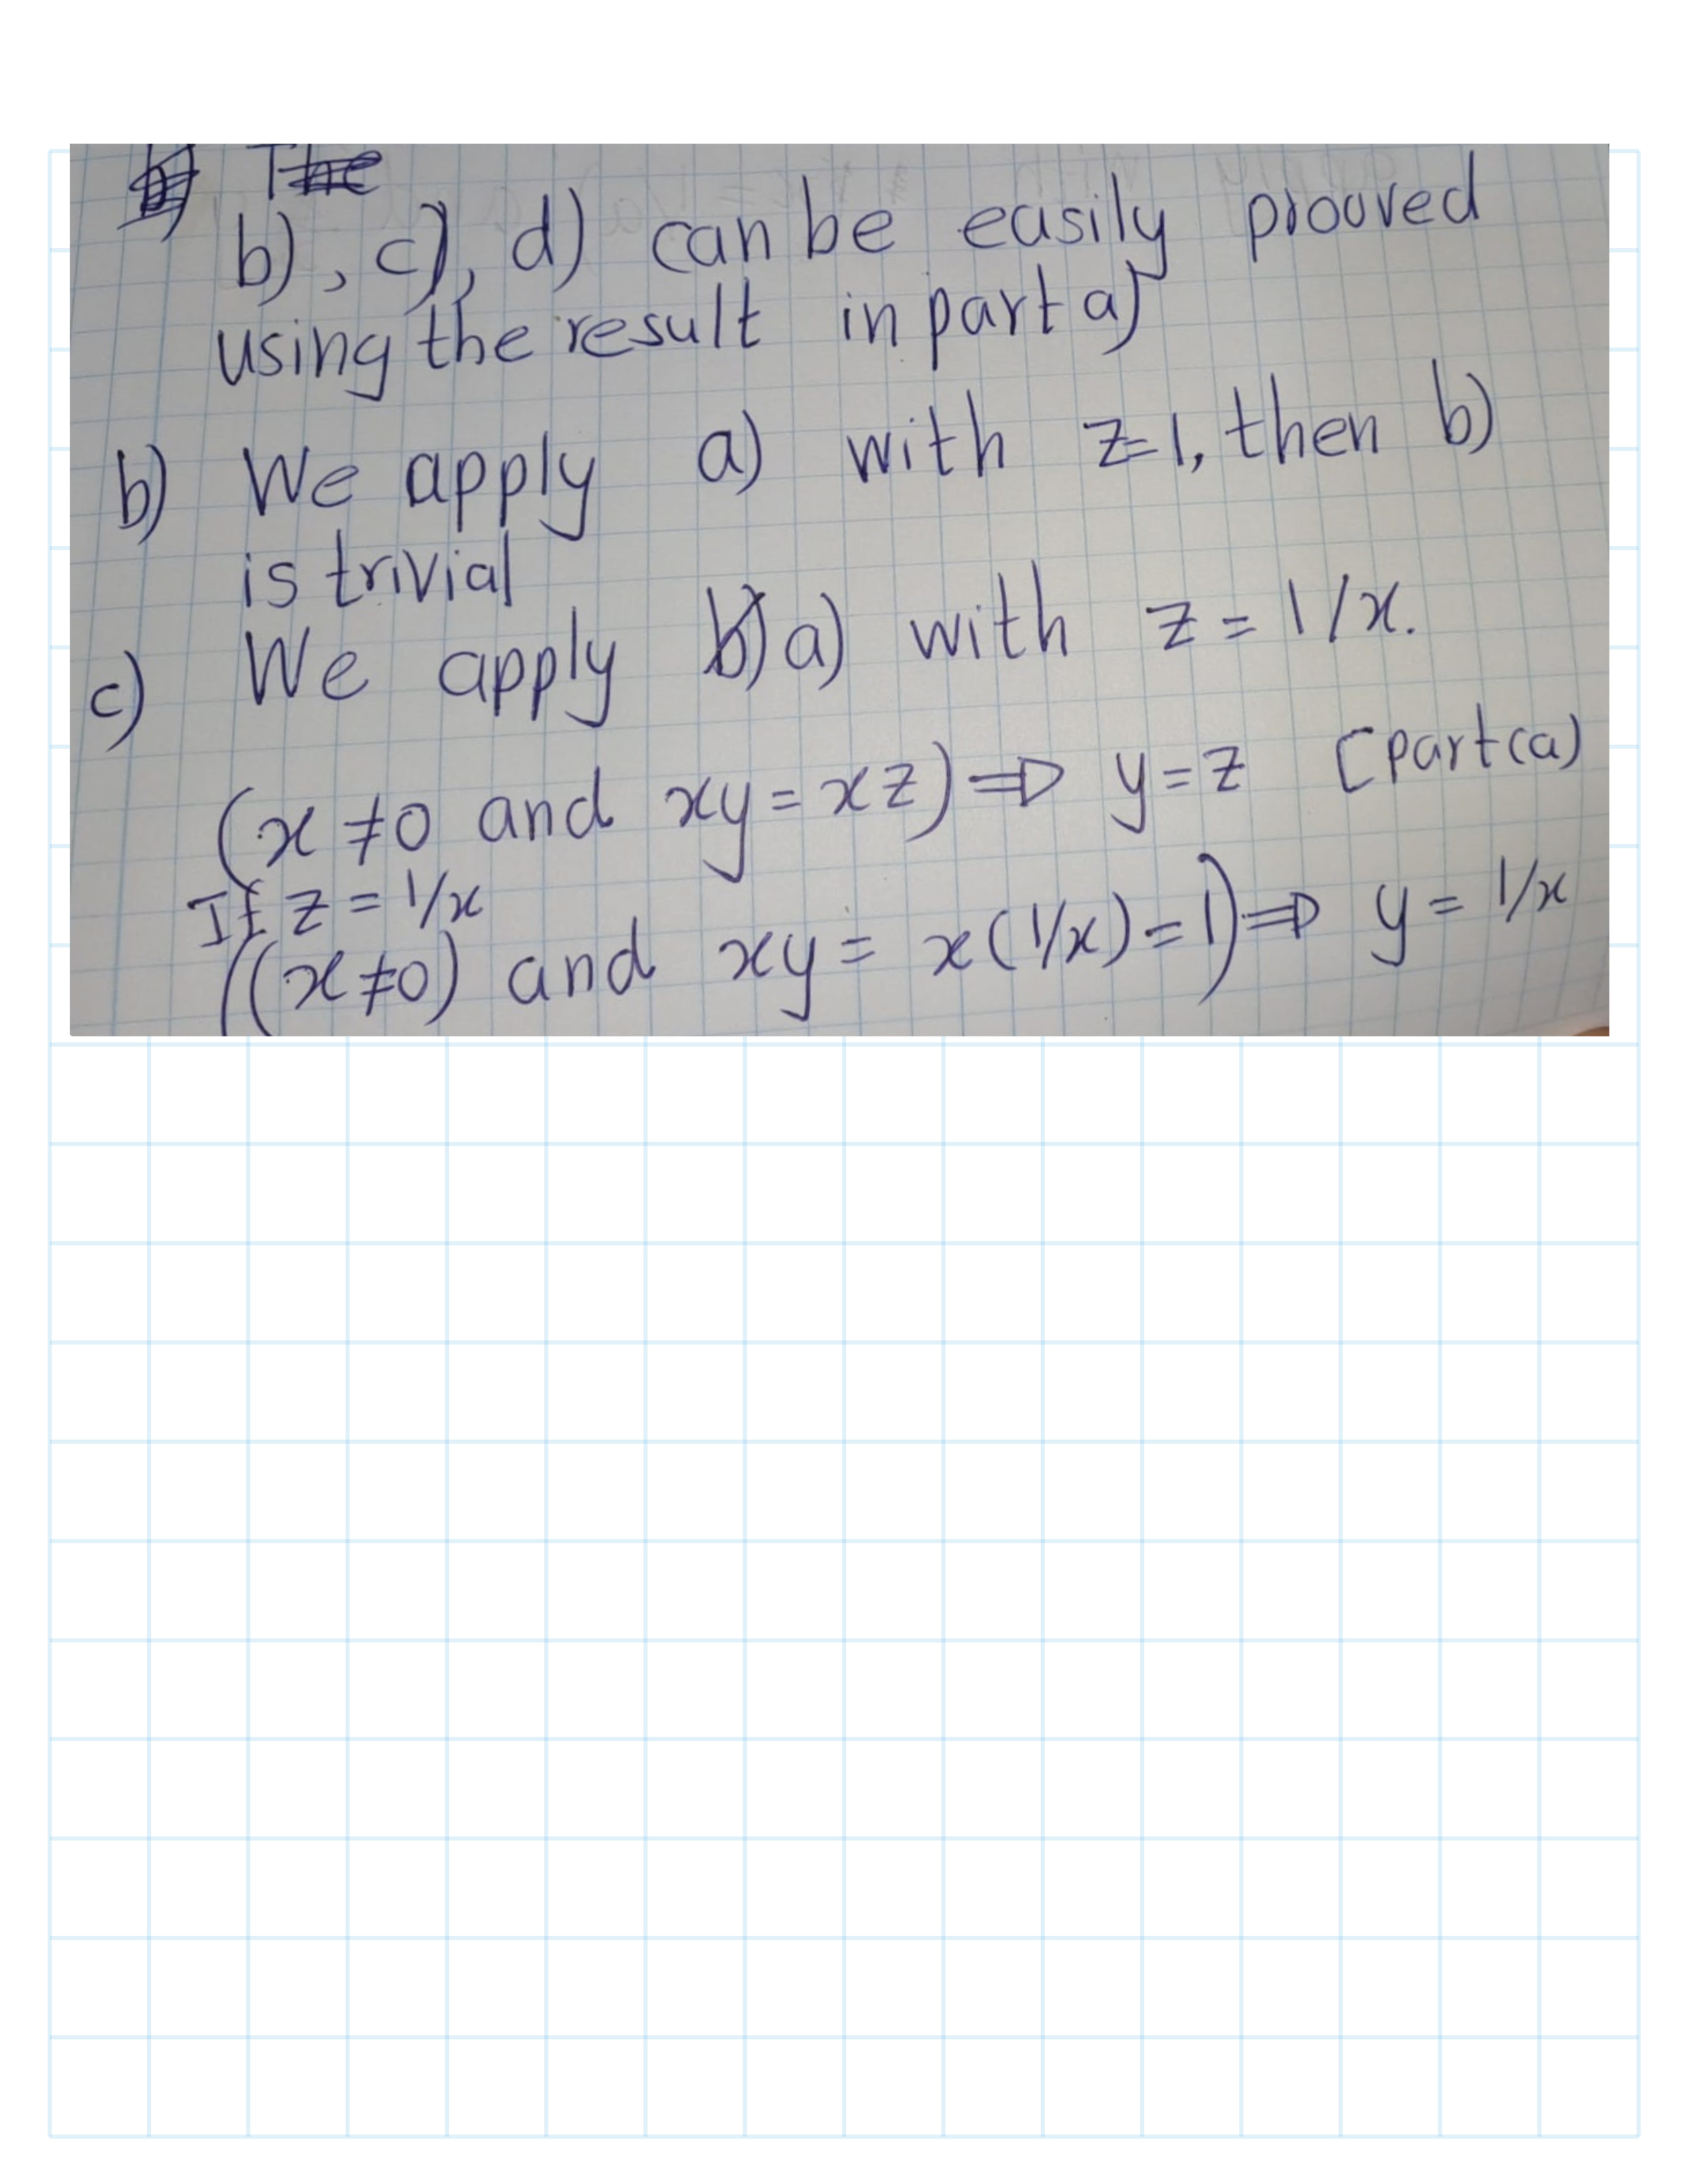
\includegraphics{Figures/Ex-1/Rudin-Ex (2).png}
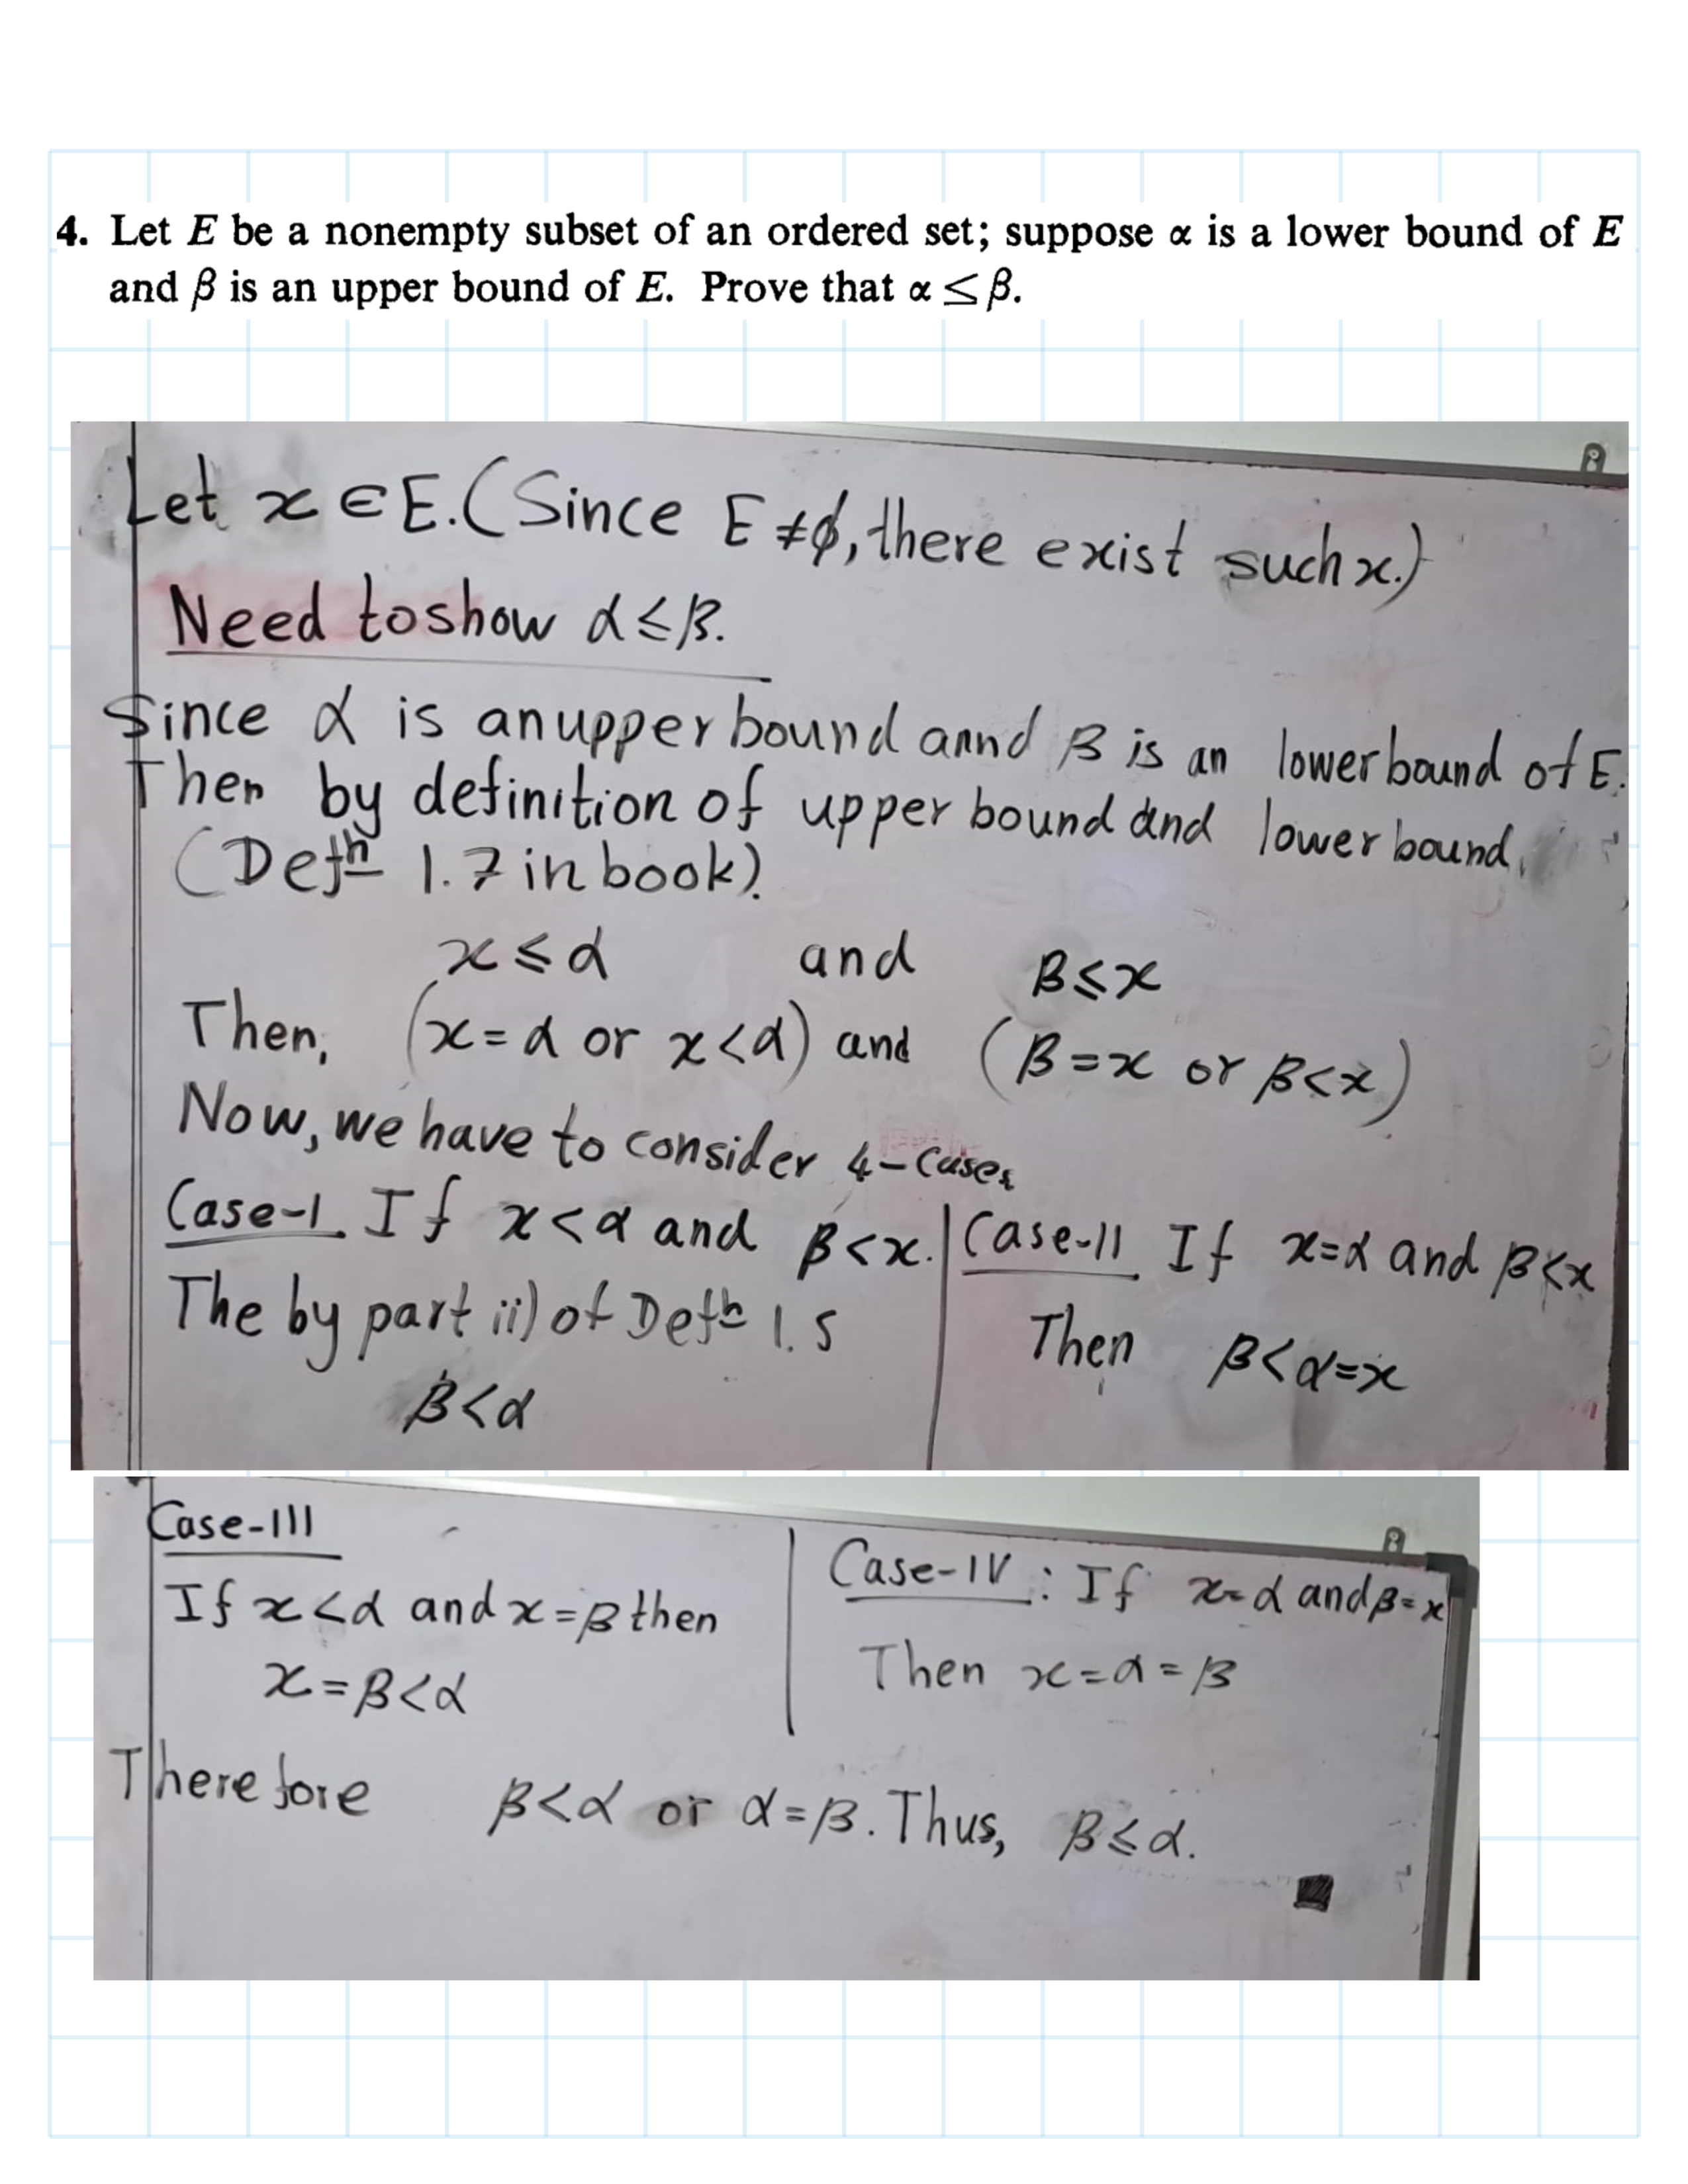
\includegraphics{Figures/Ex-1/Rudin-Ex (3).png}
\includegraphics{Figures/Ex-1/Rudin-Ex (4).png}
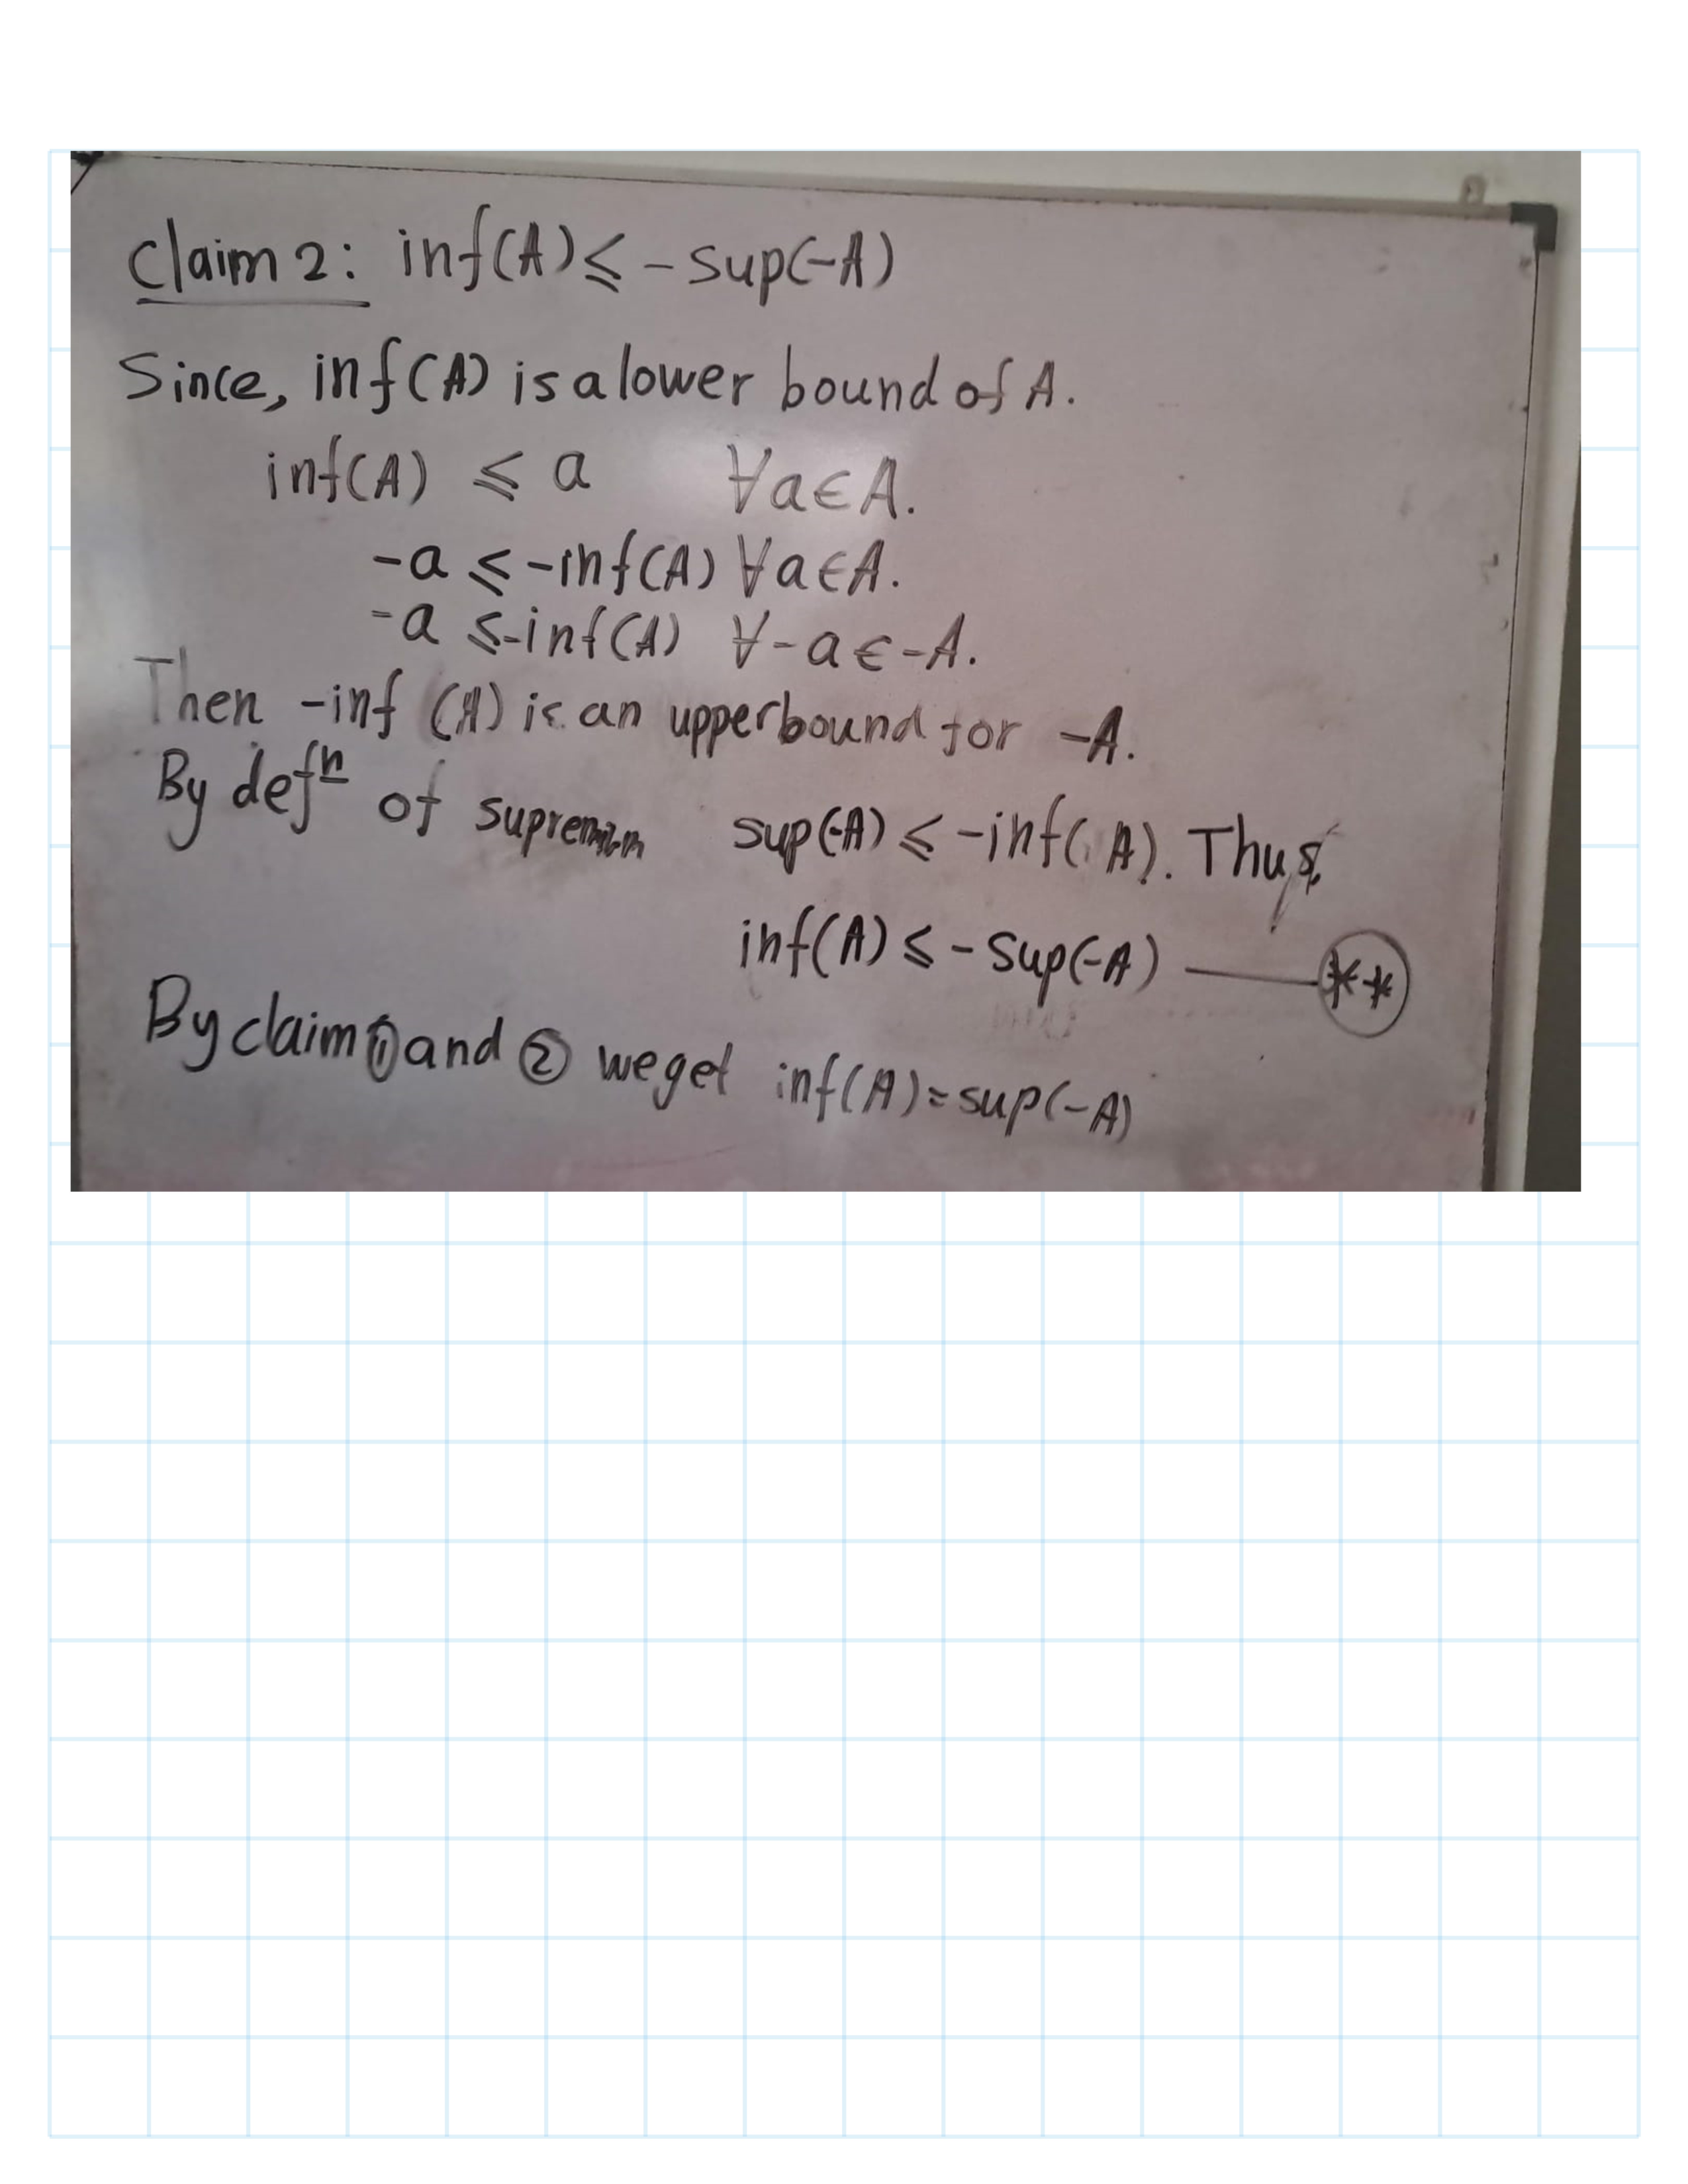
\includegraphics{Figures/Ex-1/Rudin-Ex (5).png}
\includegraphics{Figures/Ex-1/Rudin-Ex (6).png}
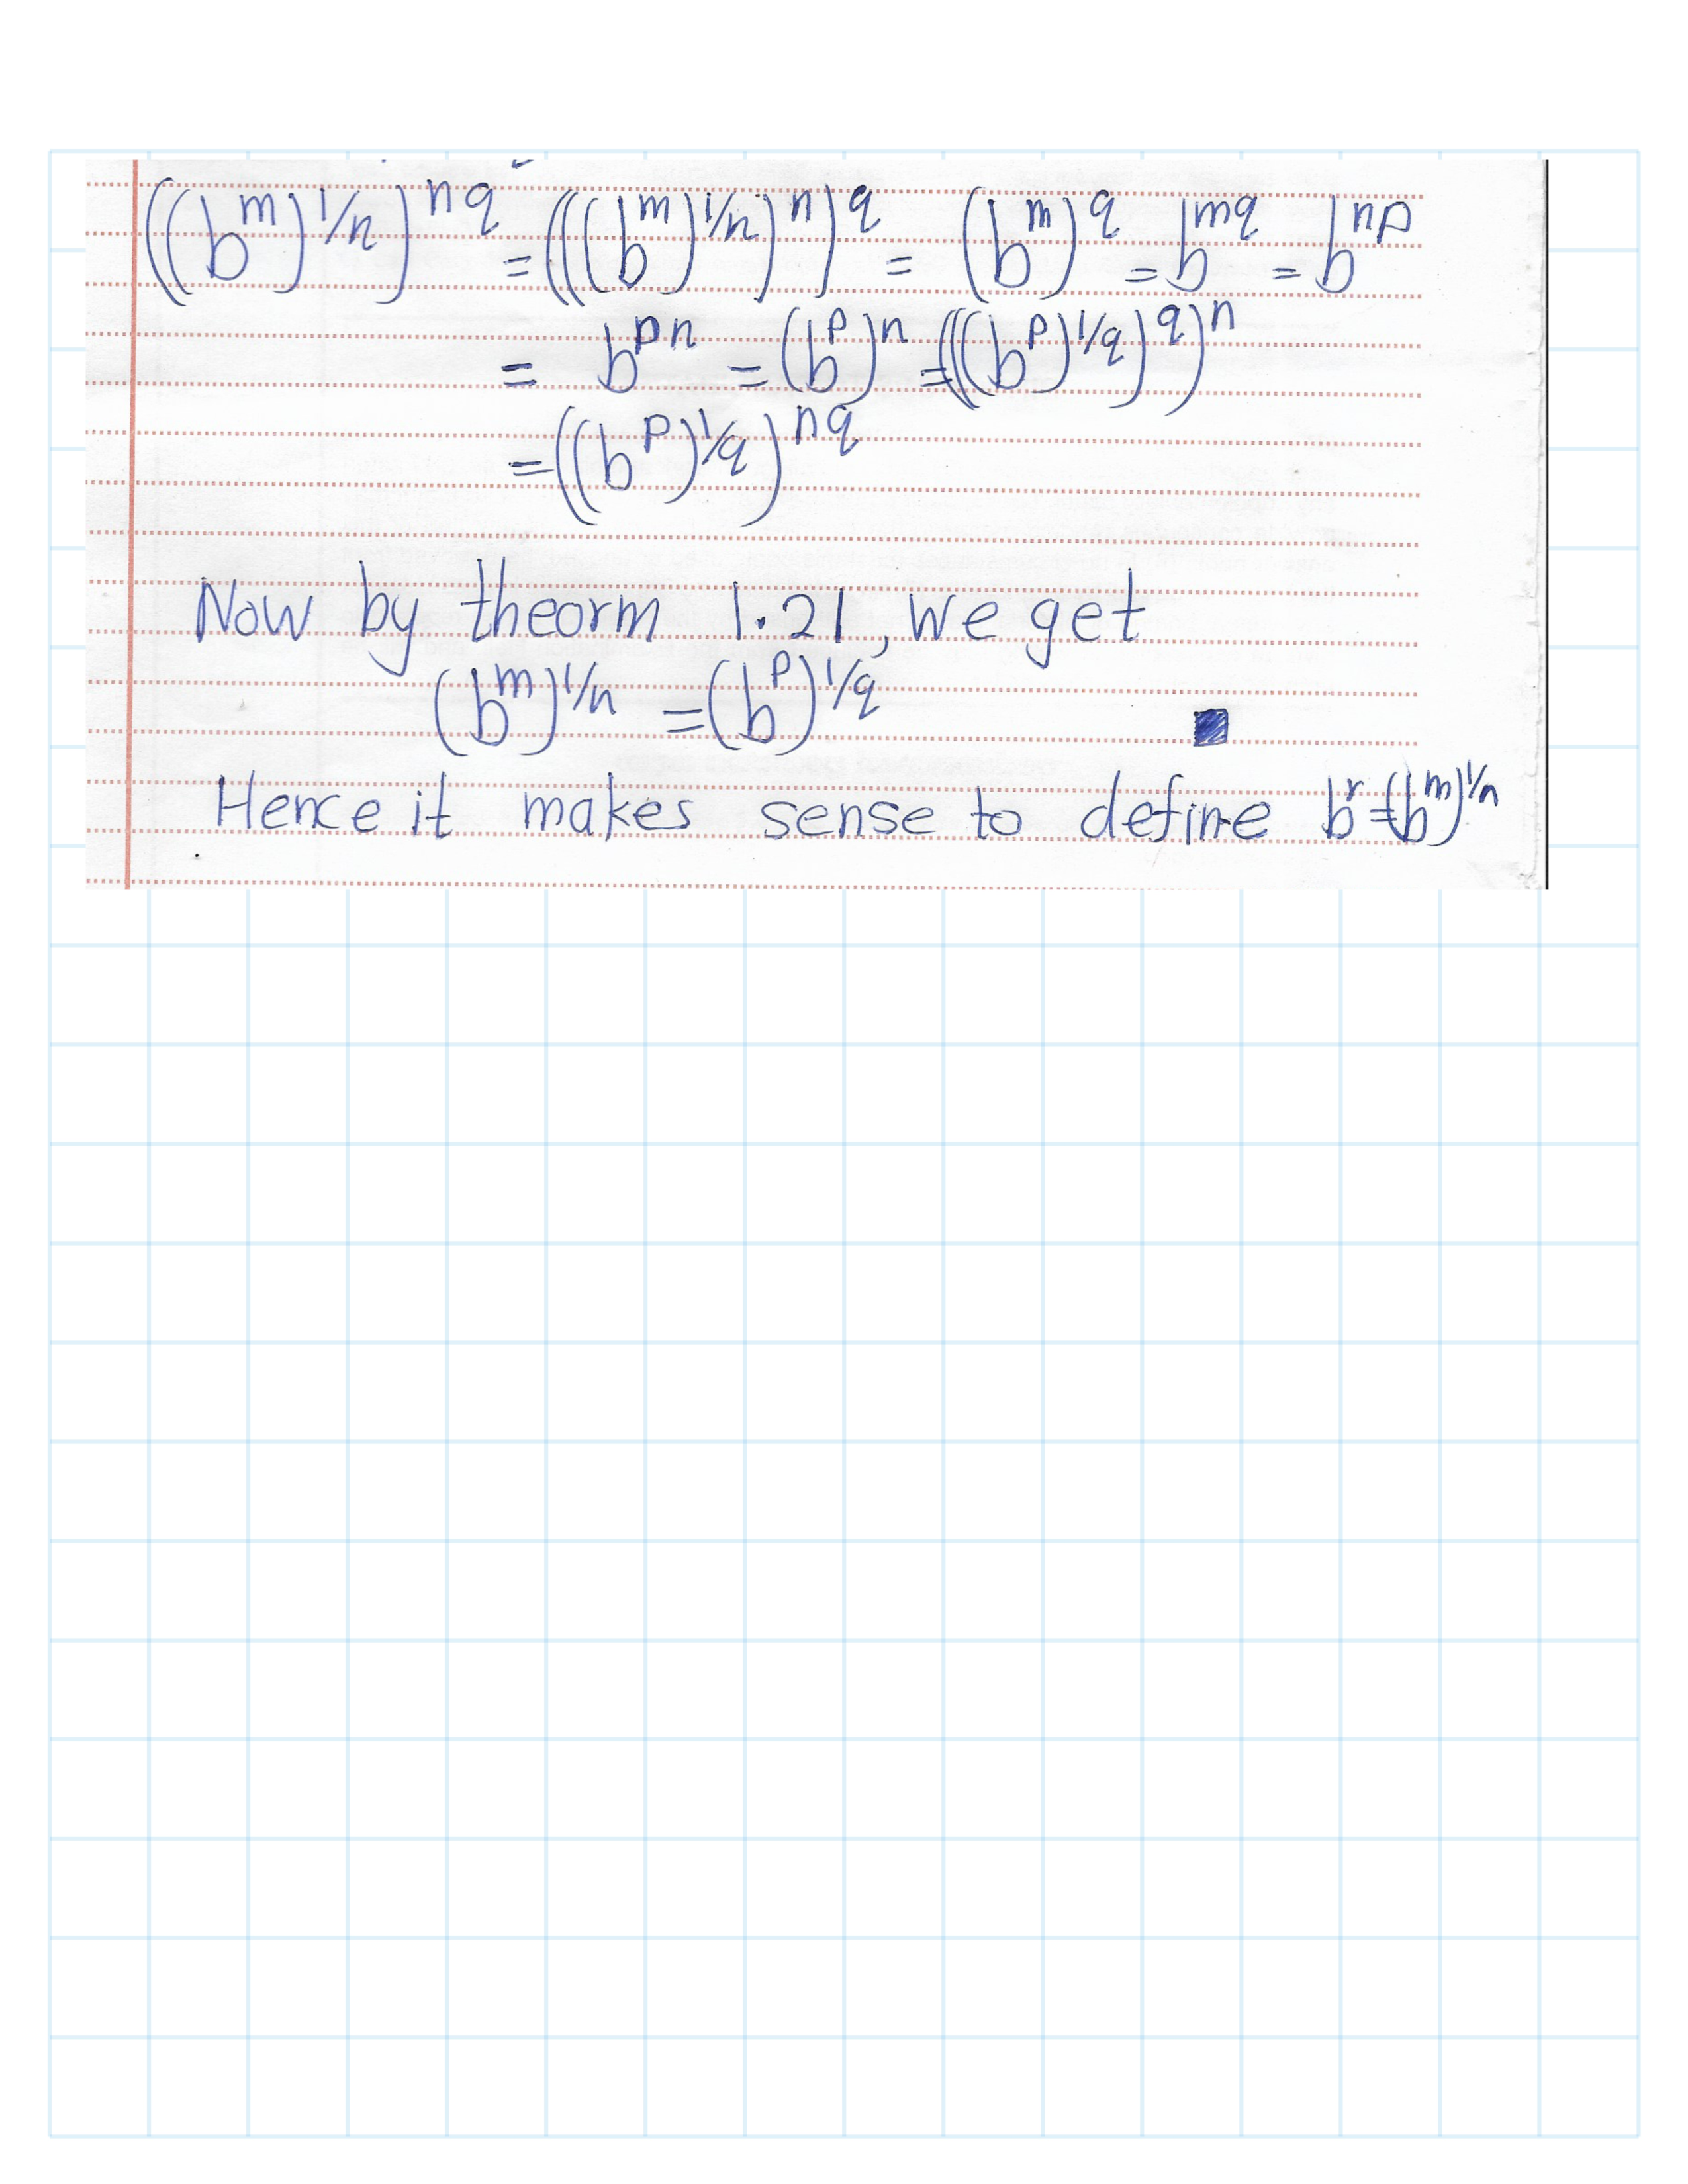
\includegraphics{Figures/Ex-1/Rudin-Ex (7).png}
\includegraphics{Figures/Ex-1/Rudin-Ex (8).png}
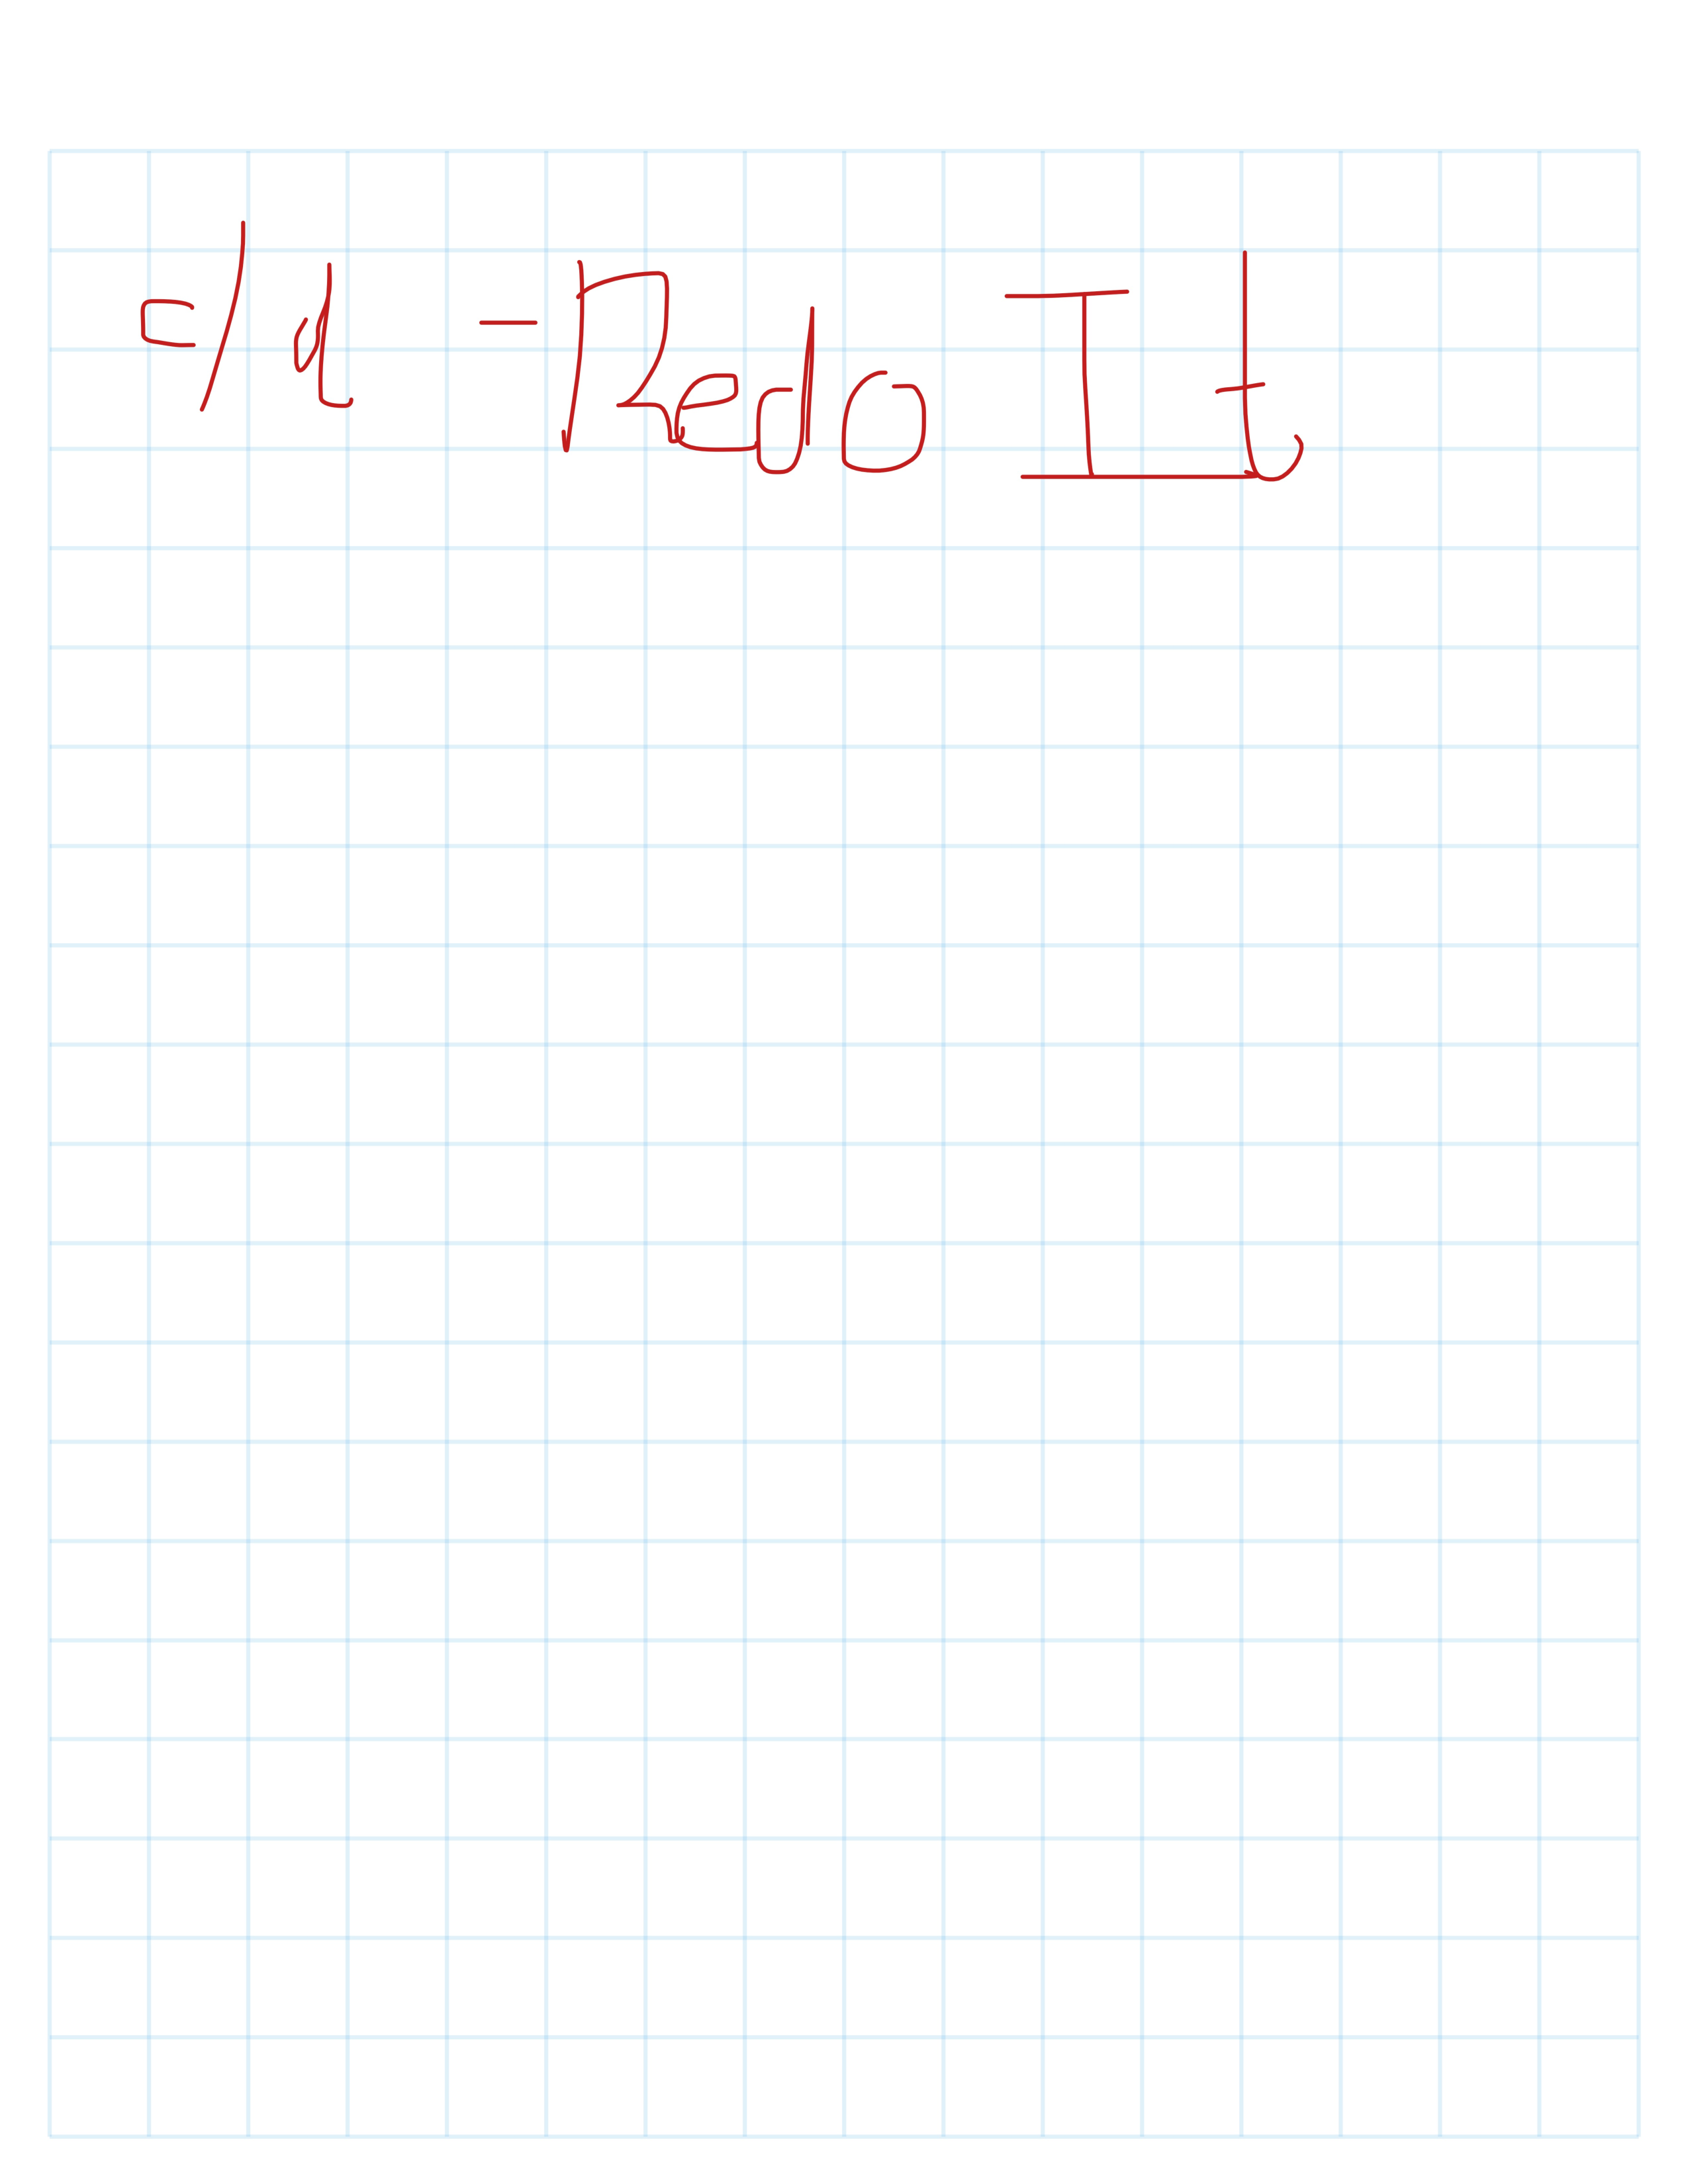
\includegraphics{Figures/Ex-1/Rudin-Ex (9).png}
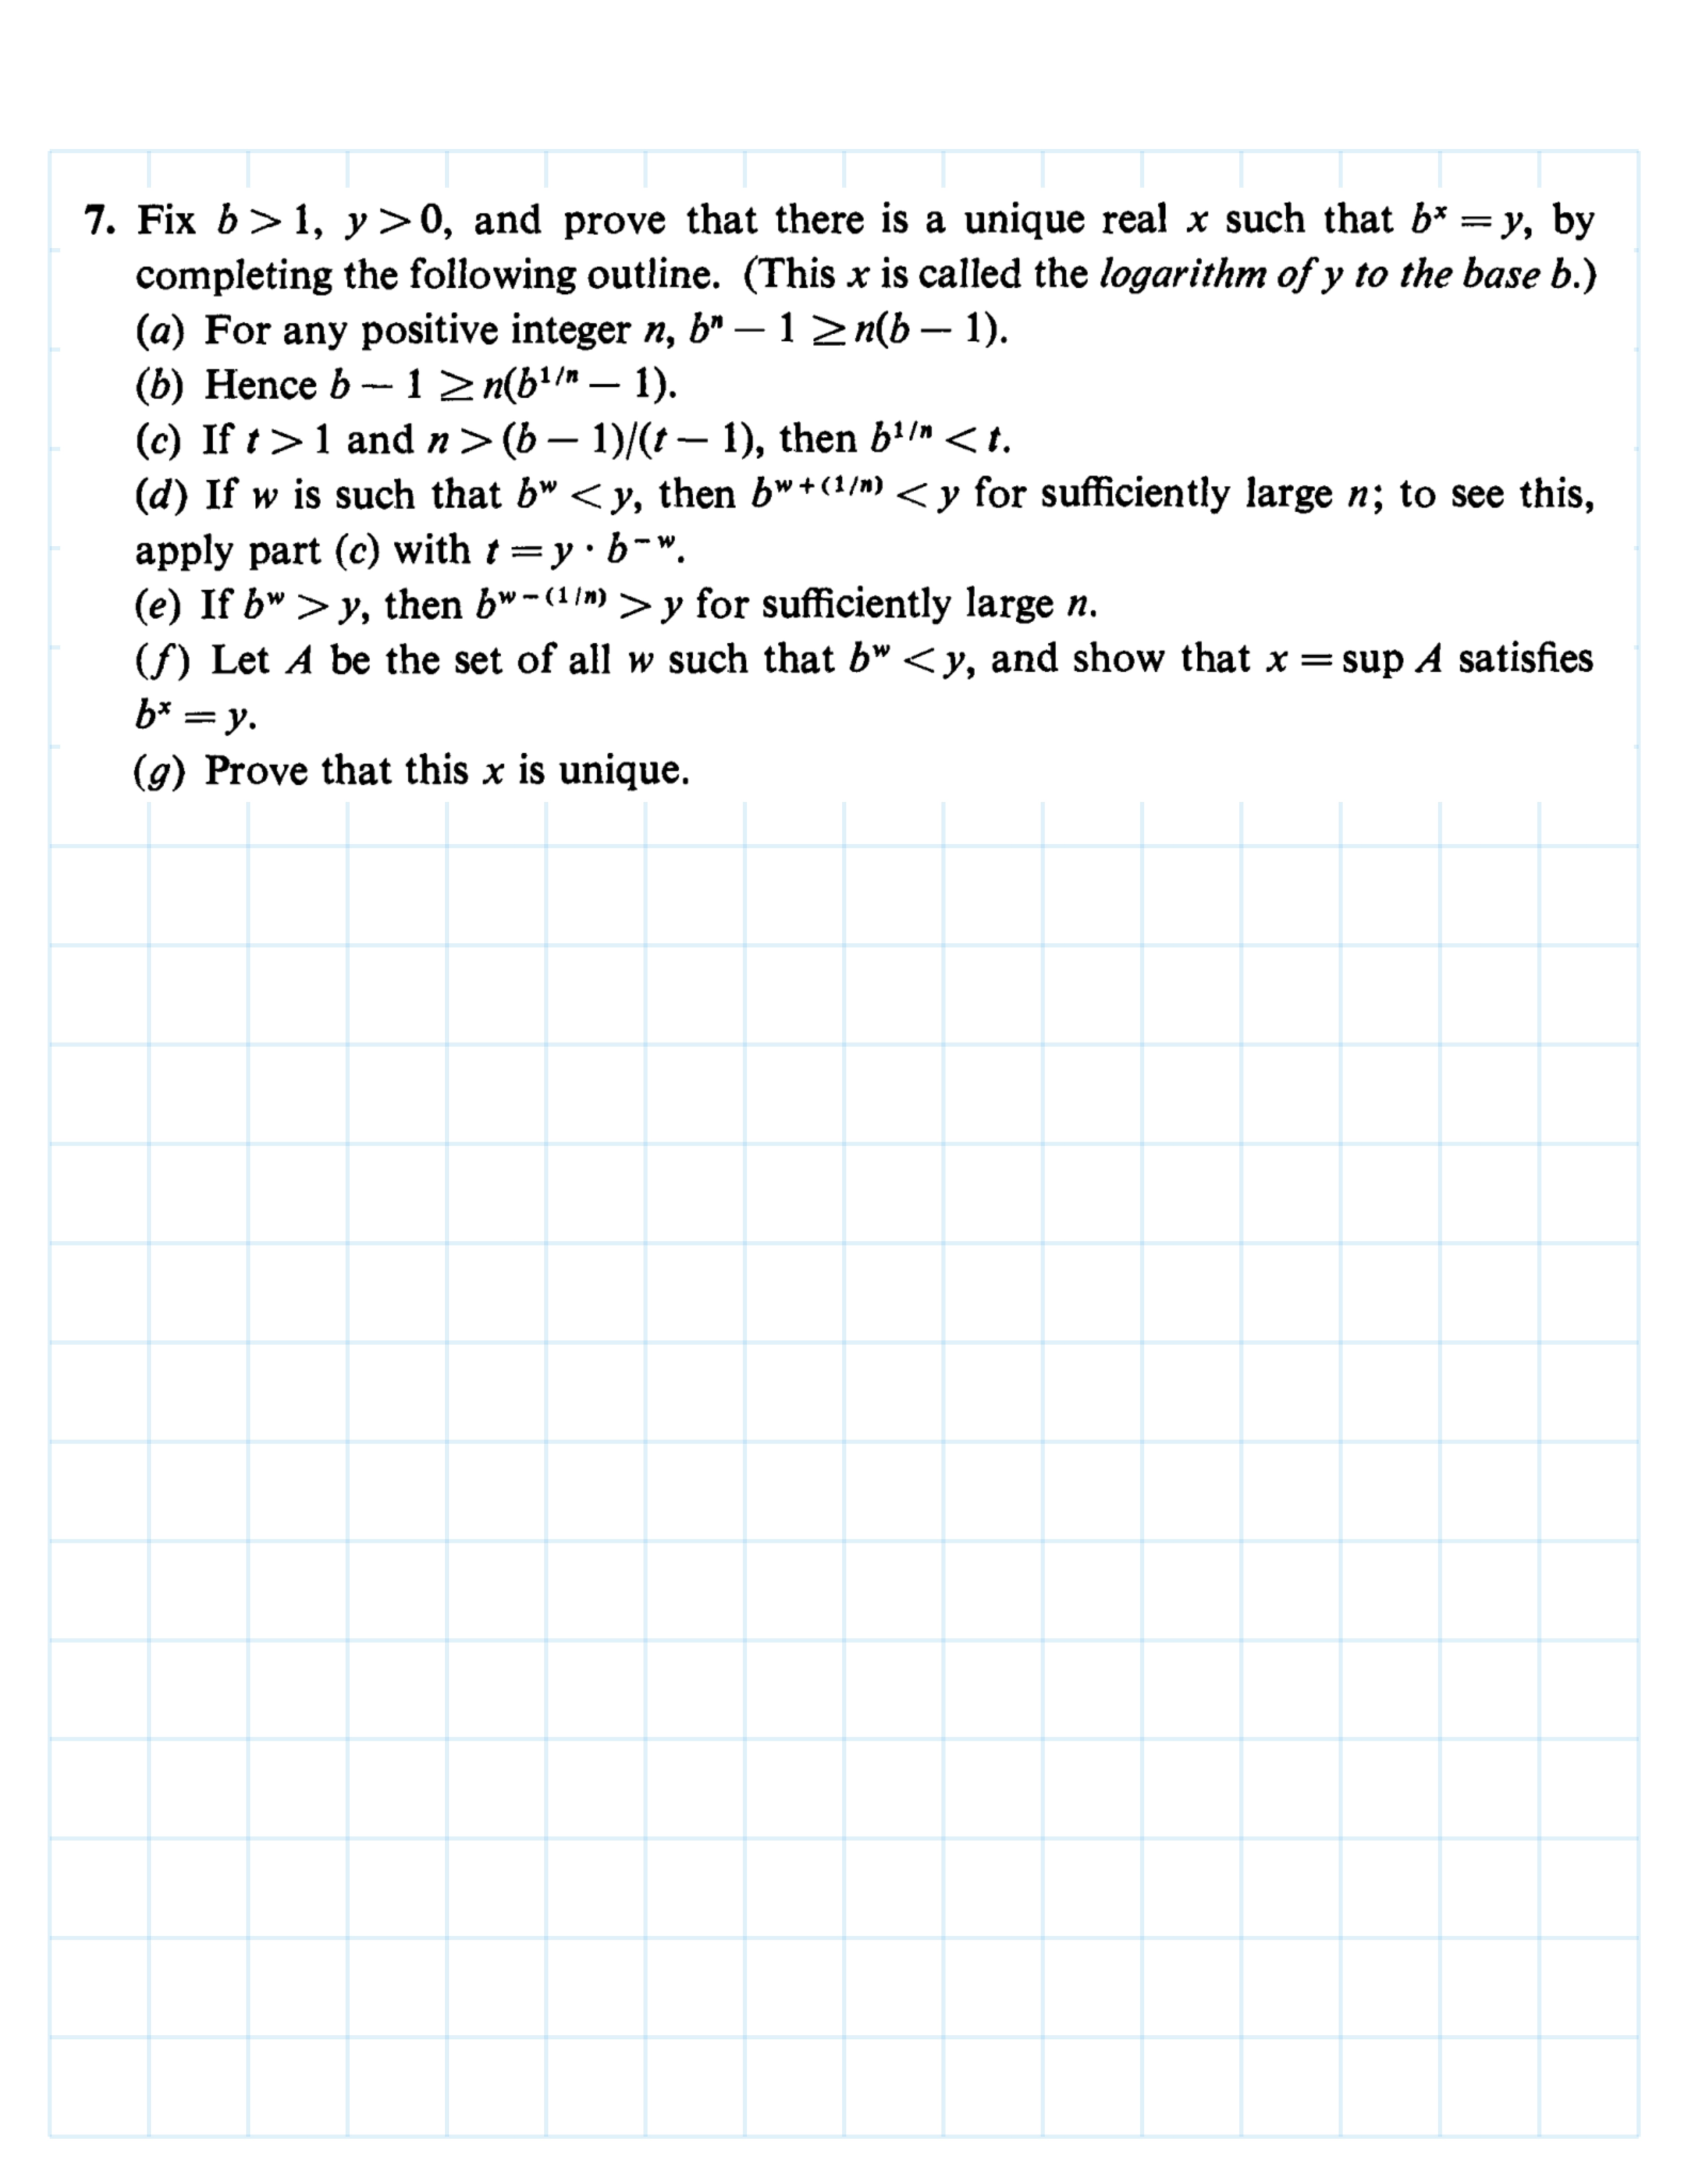
\includegraphics{Figures/Ex-1/Rudin-Ex (10).png}
\includegraphics{Figures/Ex-1/Rudin-Ex (11).png}
\includegraphics{Figures/Ex-1/Rudin-Ex (12).png}
\includegraphics{Figures/Ex-1/Rudin-Ex (13).png}
\includegraphics{Figures/Ex-1/Rudin-Ex (14).png}
\includegraphics{Figures/Ex-1/Rudin-Ex (15).png}
\includegraphics{Figures/Ex-1/Rudin-Ex (16).png}
\includegraphics{Figures/Ex-1/Rudin-Ex (17).png}
\includegraphics{Figures/Ex-1/Rudin-Ex (18).png}
\includegraphics{Figures/Ex-1/Rudin-Ex (19).png}
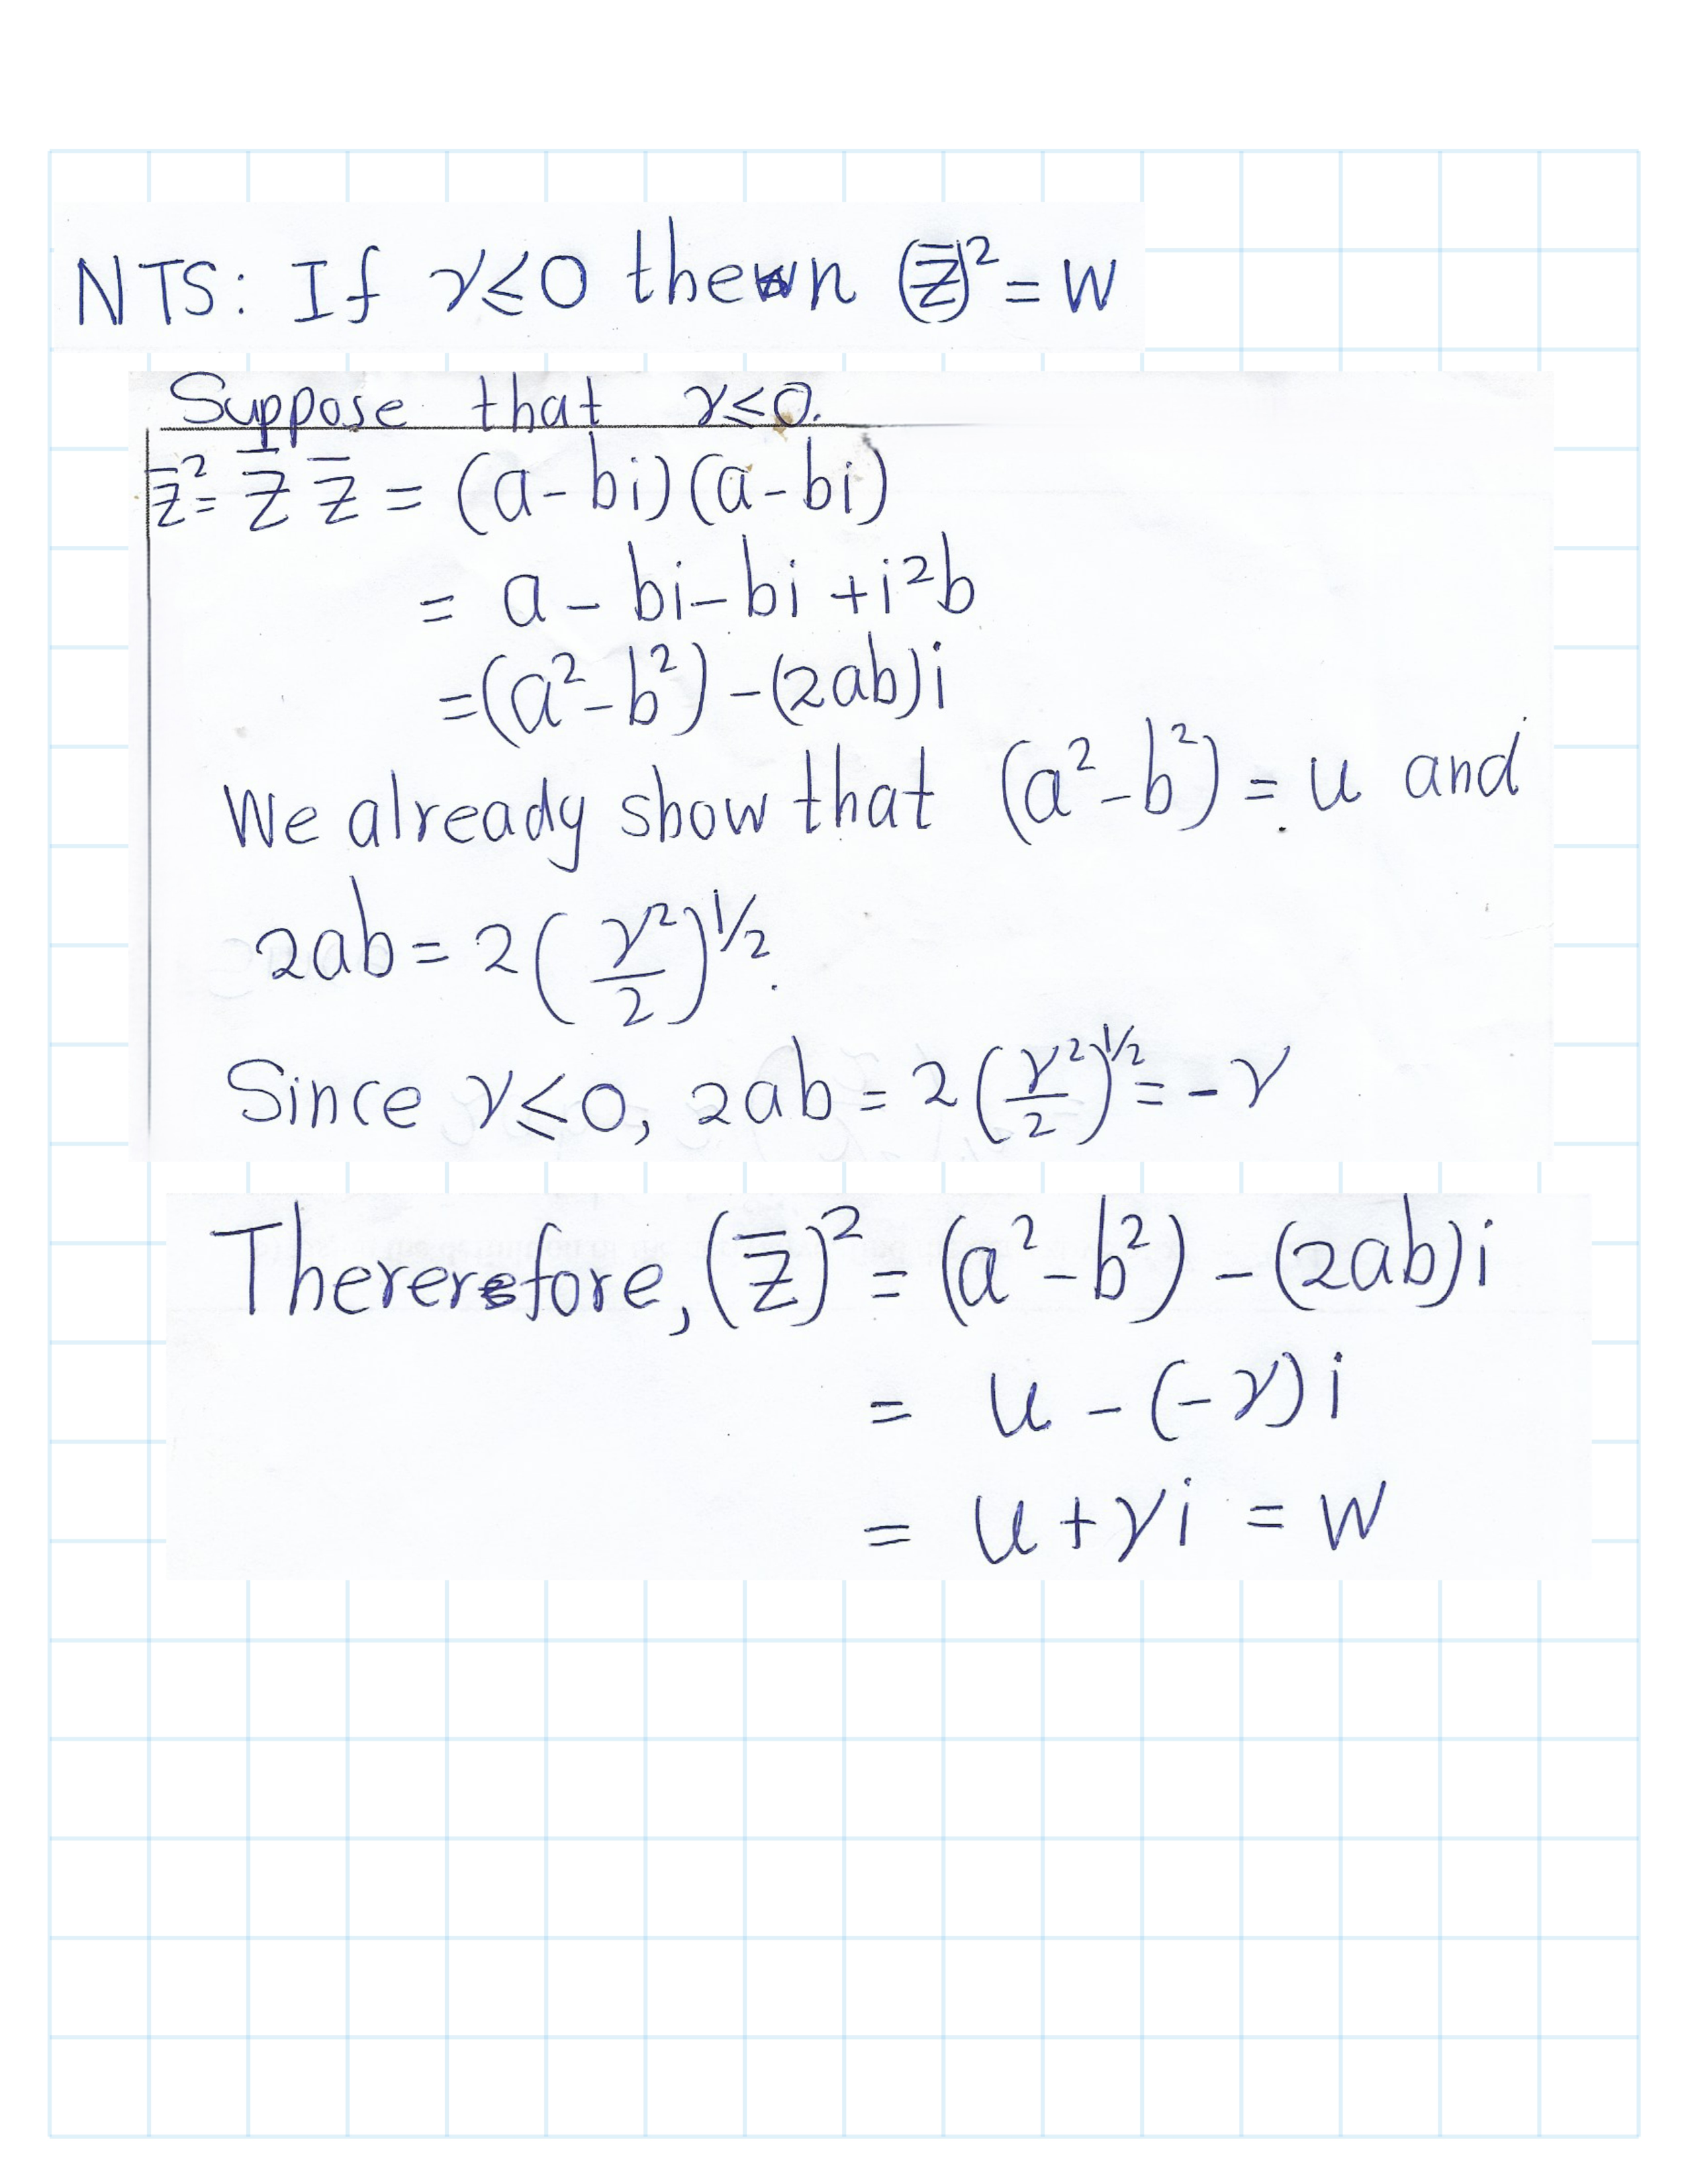
\includegraphics{Figures/Ex-1/Rudin-Ex (20).png}
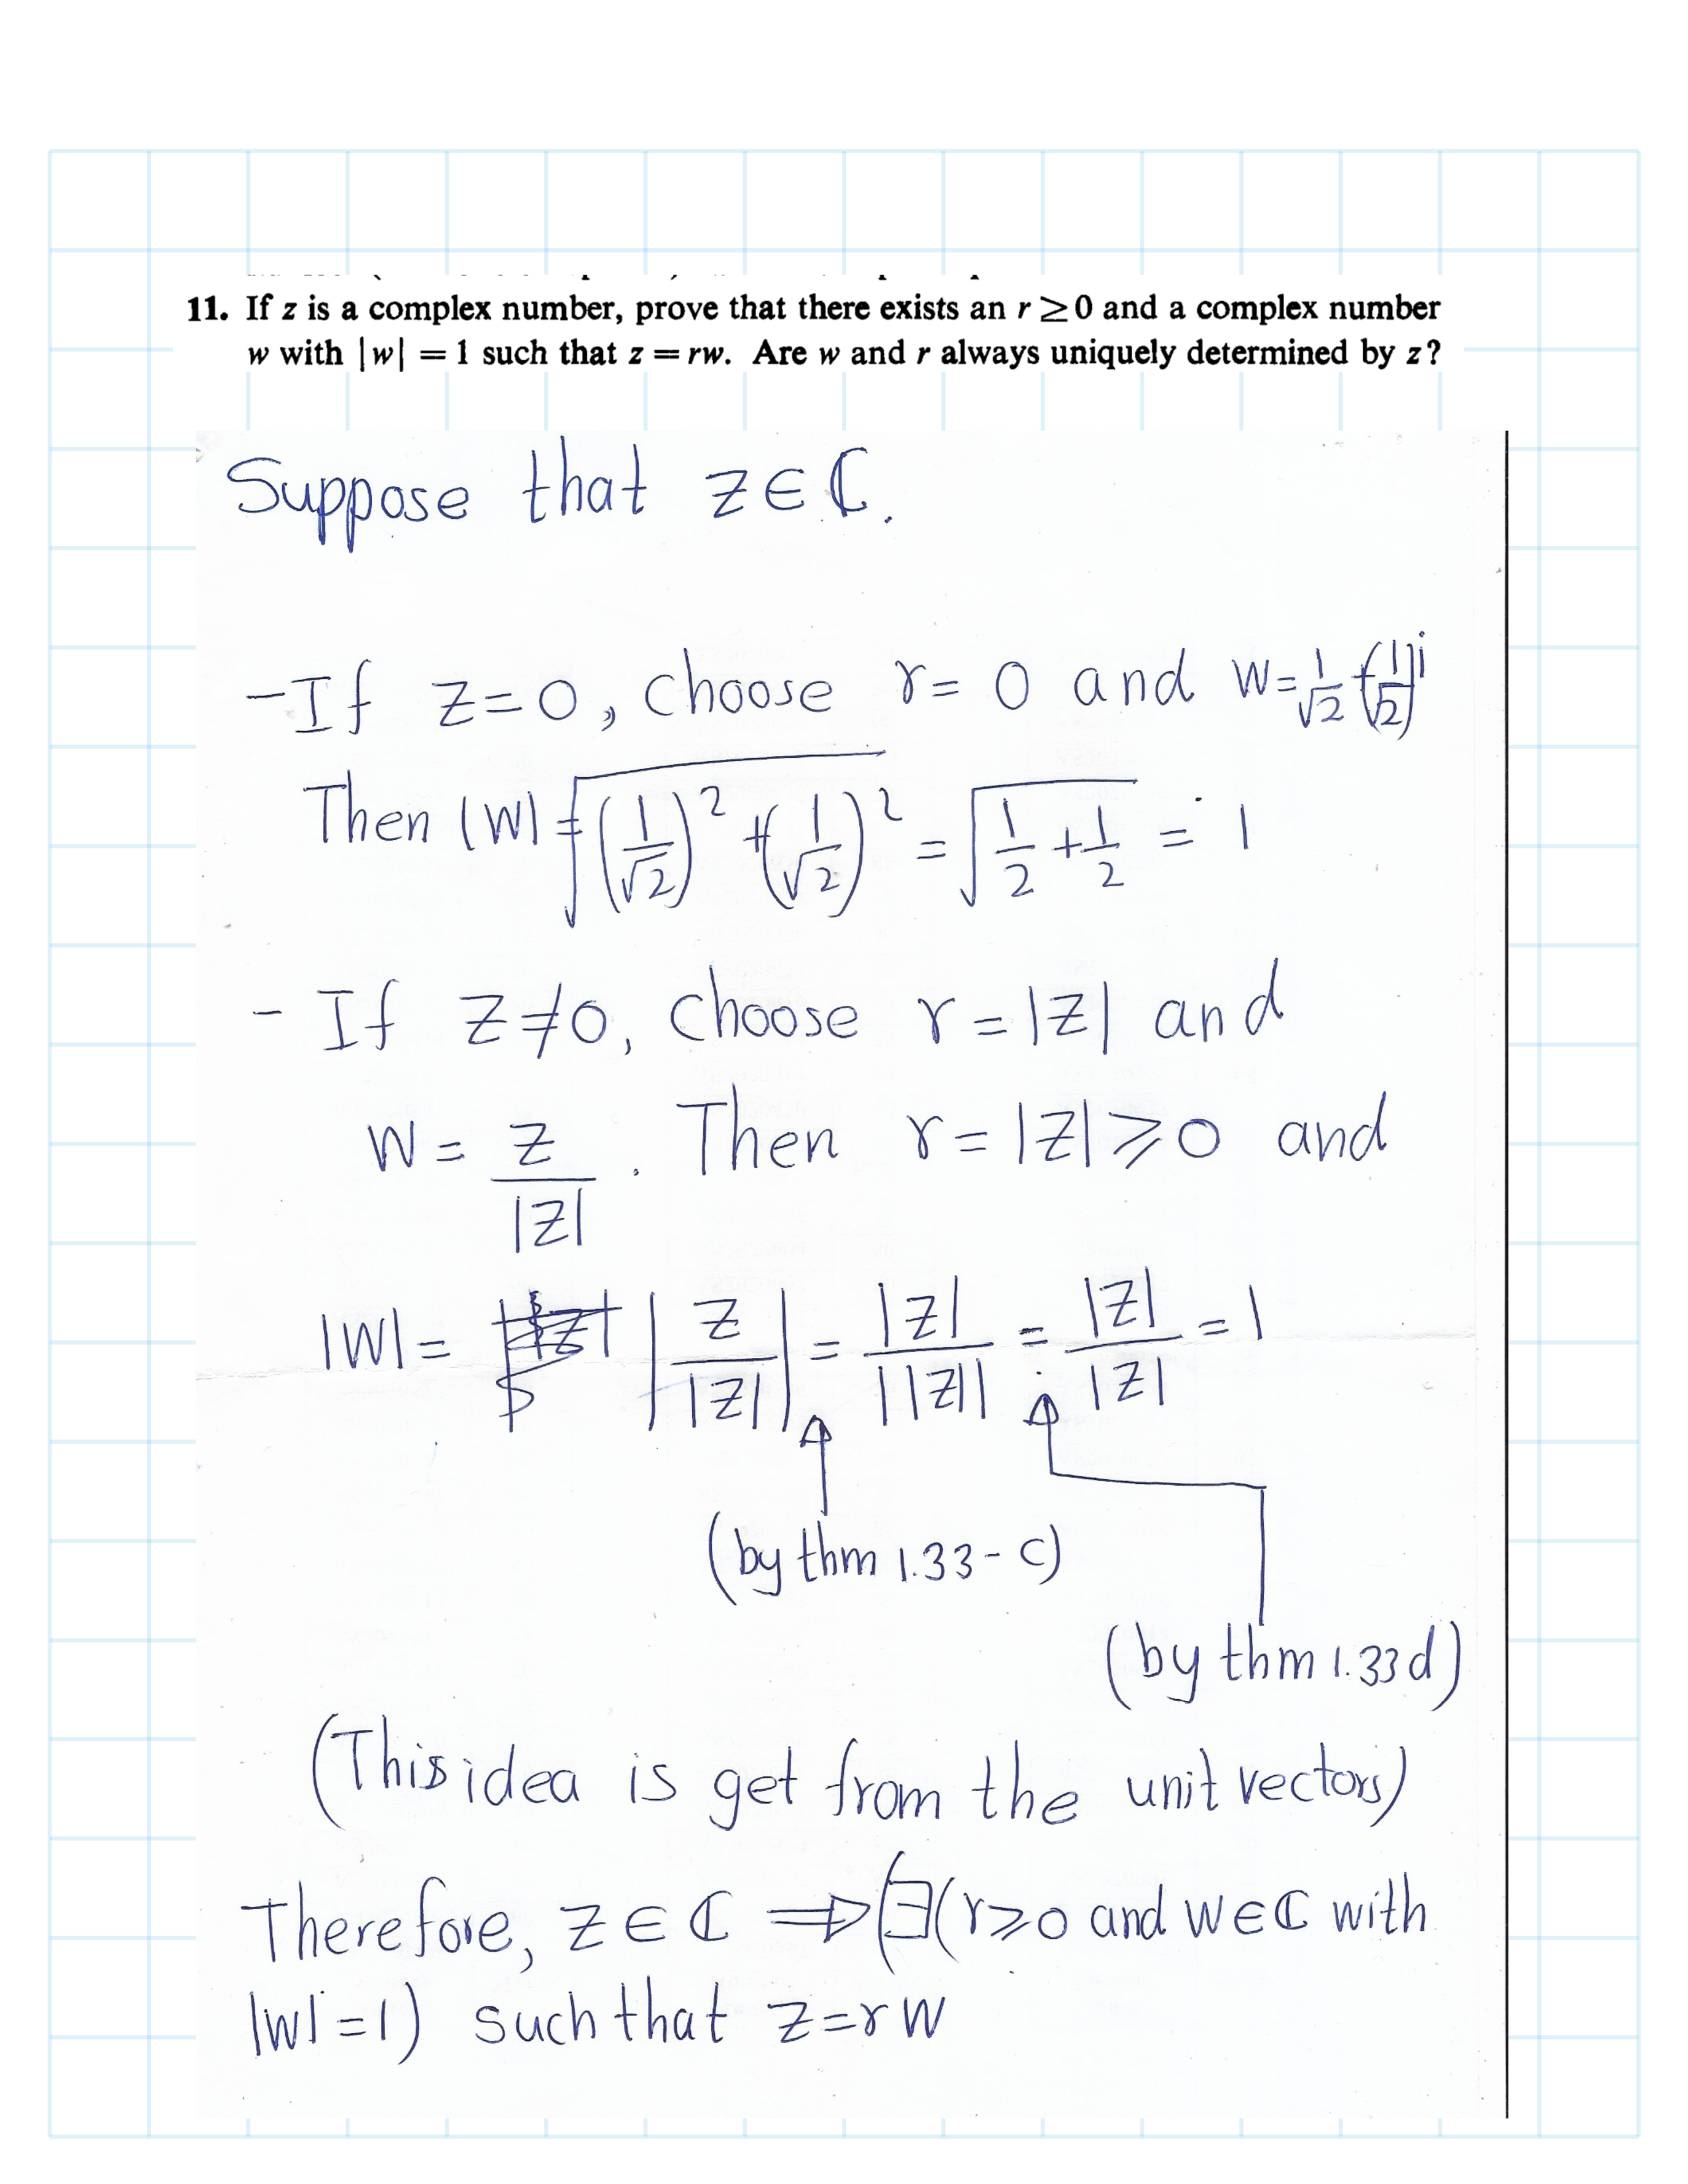
\includegraphics{Figures/Ex-1/Rudin-Ex (21).png}
\includegraphics{Figures/Ex-1/Rudin-Ex (22).png}
\includegraphics{Figures/Ex-1/Rudin-Ex (23).png}
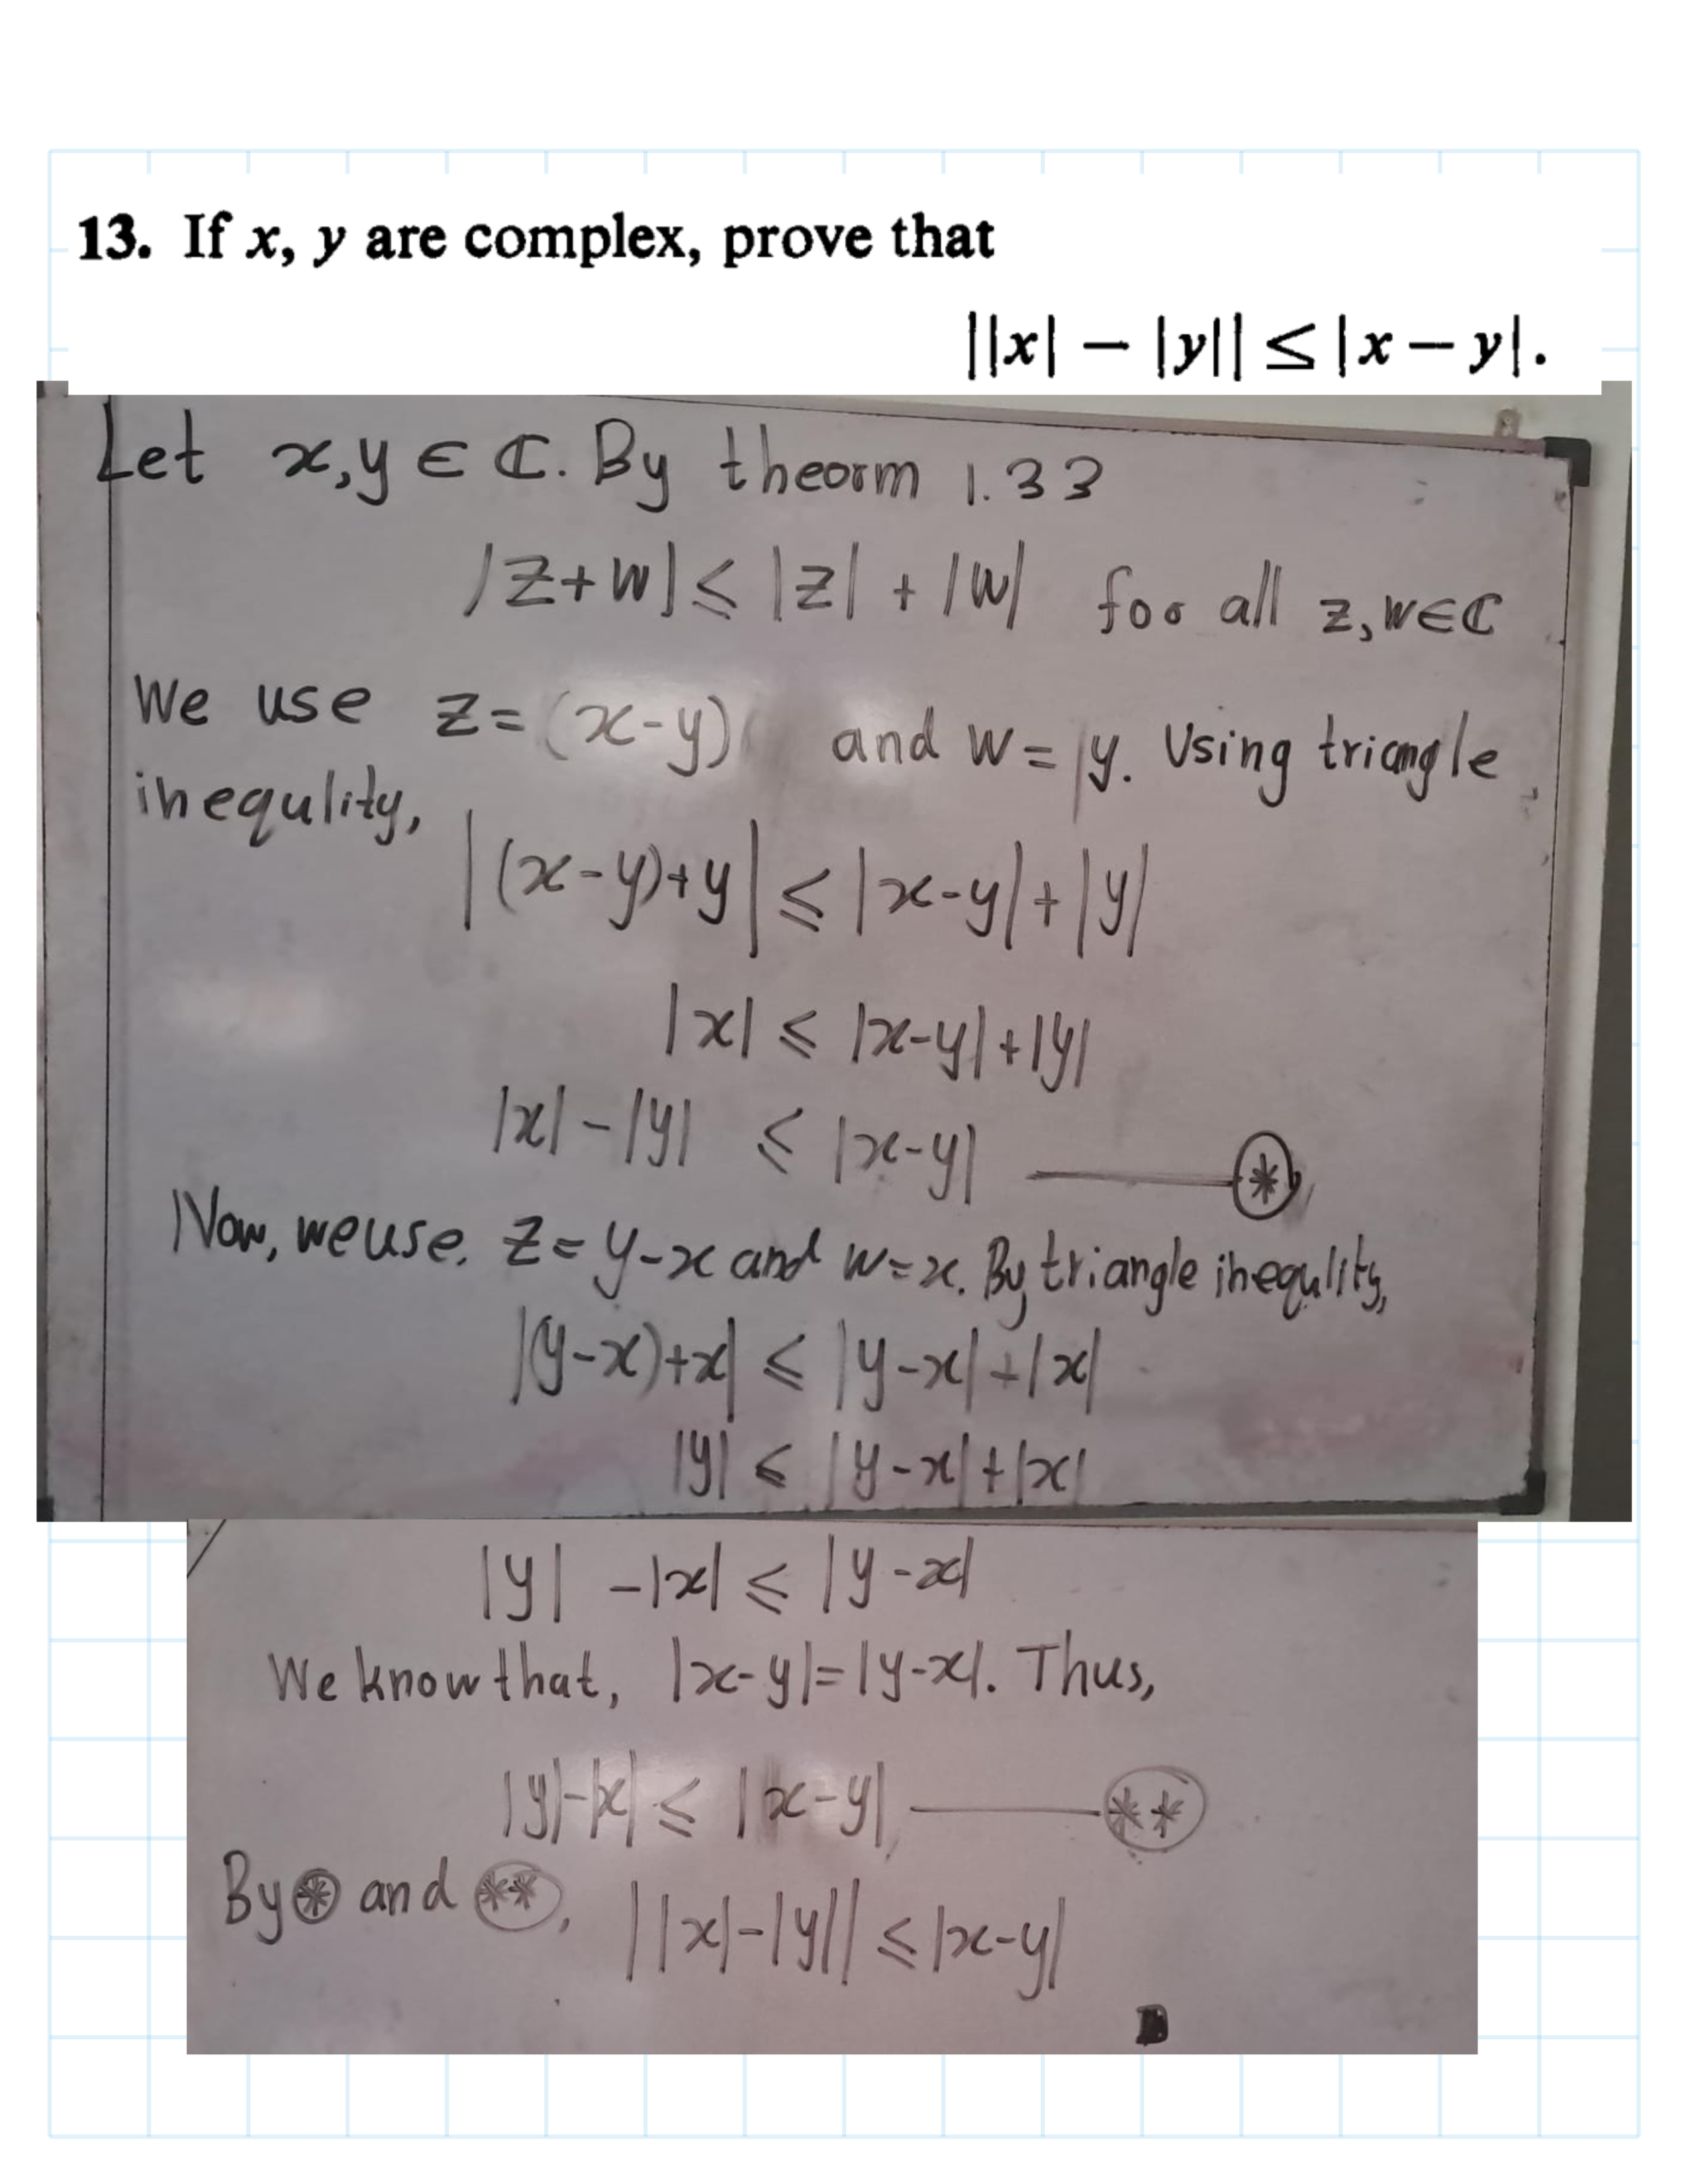
\includegraphics{Figures/Ex-1/Rudin-Ex (24).png}
\includegraphics{Figures/Ex-1/Rudin-Ex (25).png}
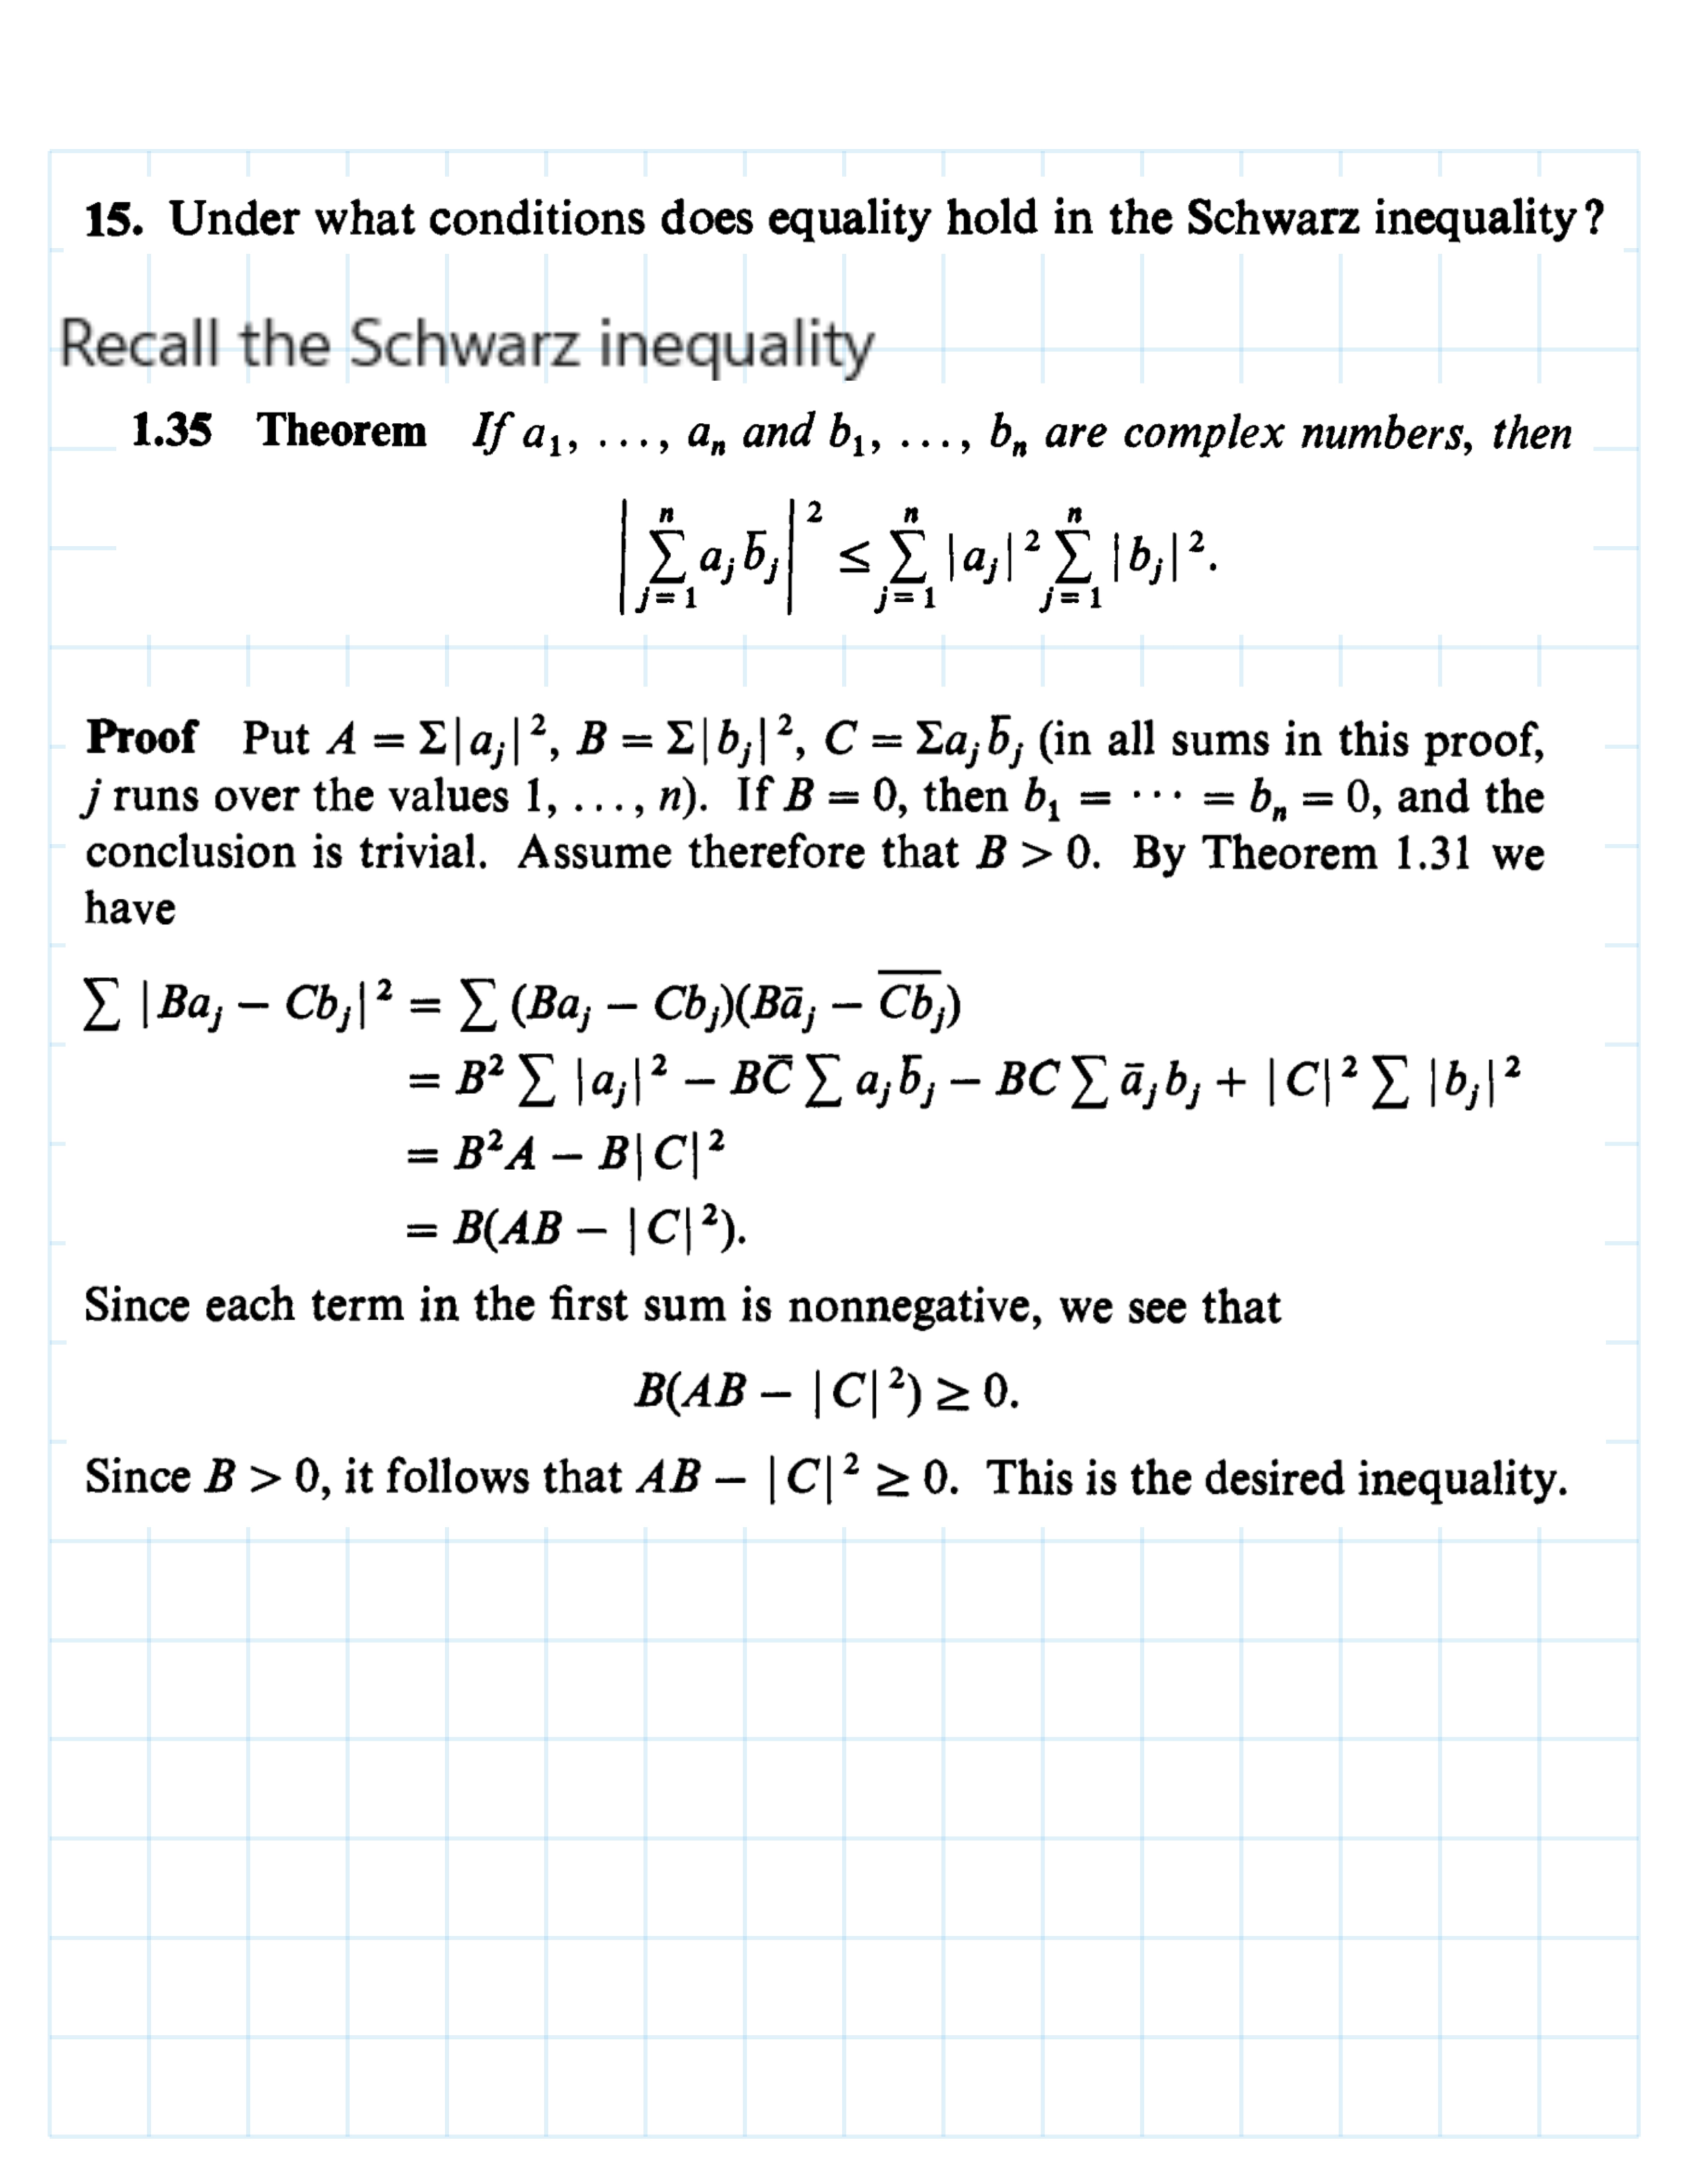
\includegraphics{Figures/Ex-1/Rudin-Ex (26).png}
\includegraphics{Figures/Ex-1/Rudin-Ex (27).png}
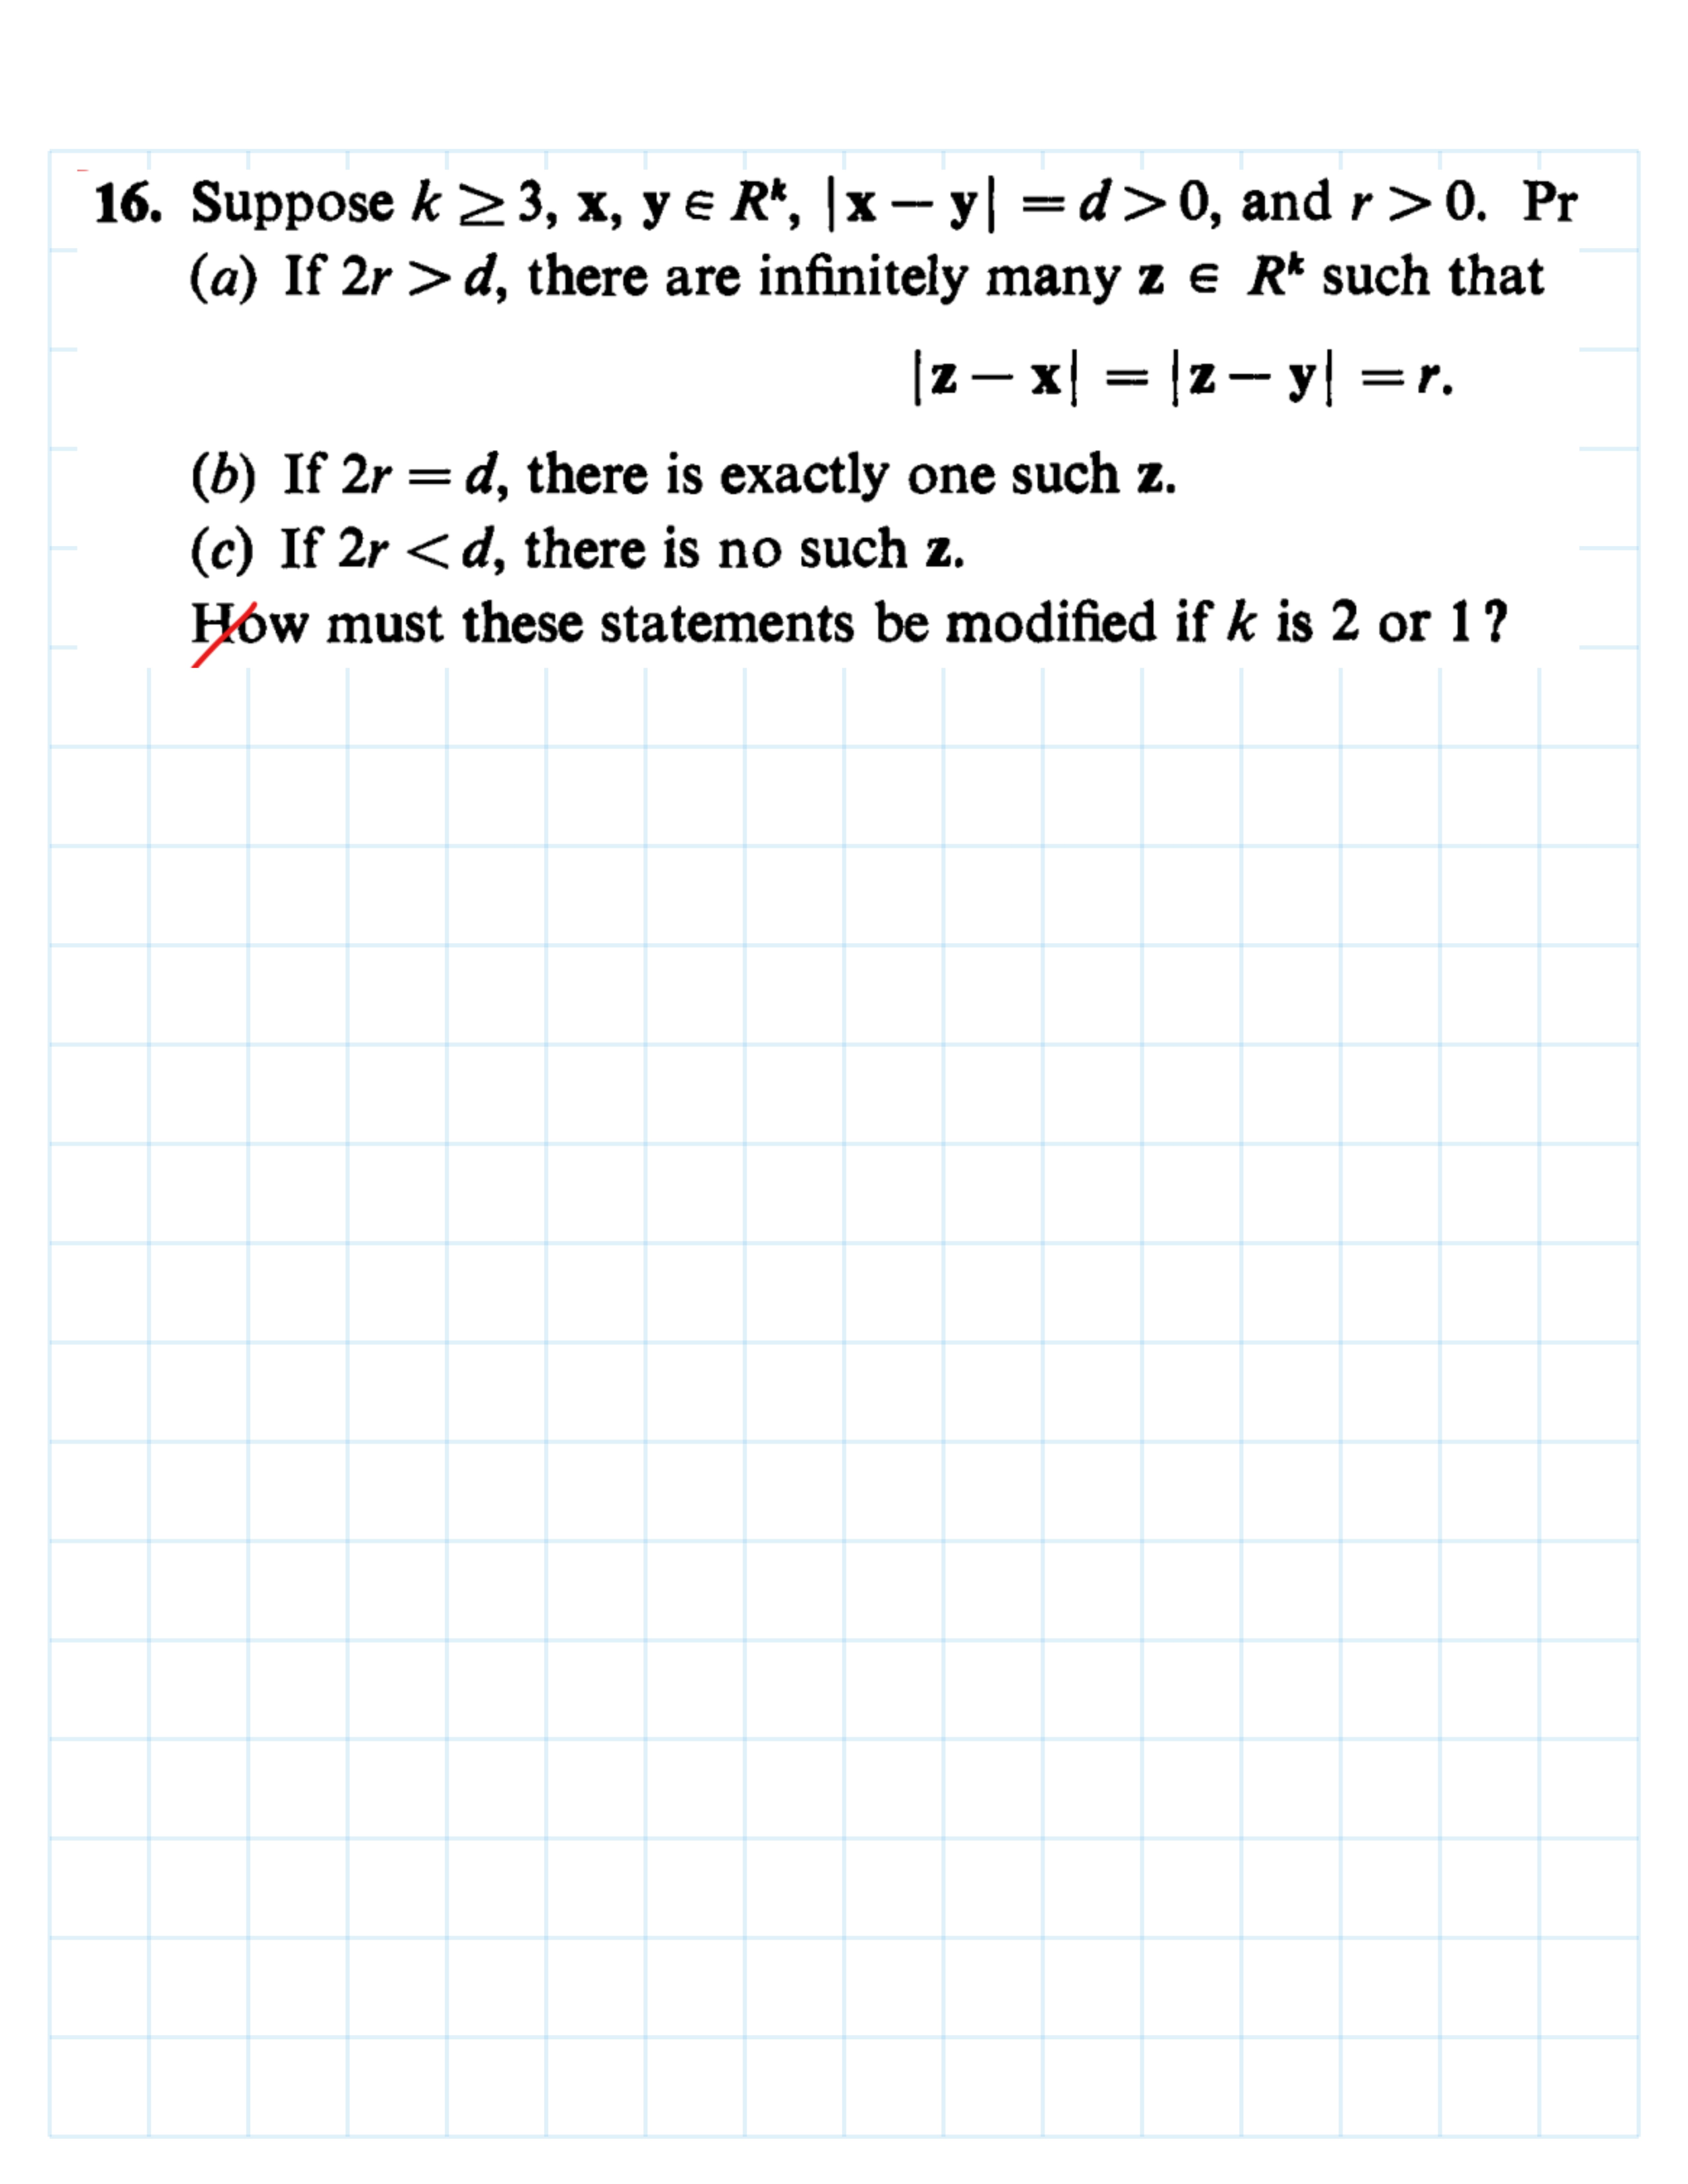
\includegraphics{Figures/Ex-1/Rudin-Ex (28).png}
\includegraphics{Figures/Ex-1/Rudin-Ex (29).png}
\includegraphics{Figures/Ex-1/Rudin-Ex (30).png}
\includegraphics{Figures/Ex-1/Rudin-Ex (31).png}
\includegraphics{Figures/Ex-1/Rudin-Ex (32).png}
\includegraphics{Figures/Ex-1/Rudin-Ex (33).png}
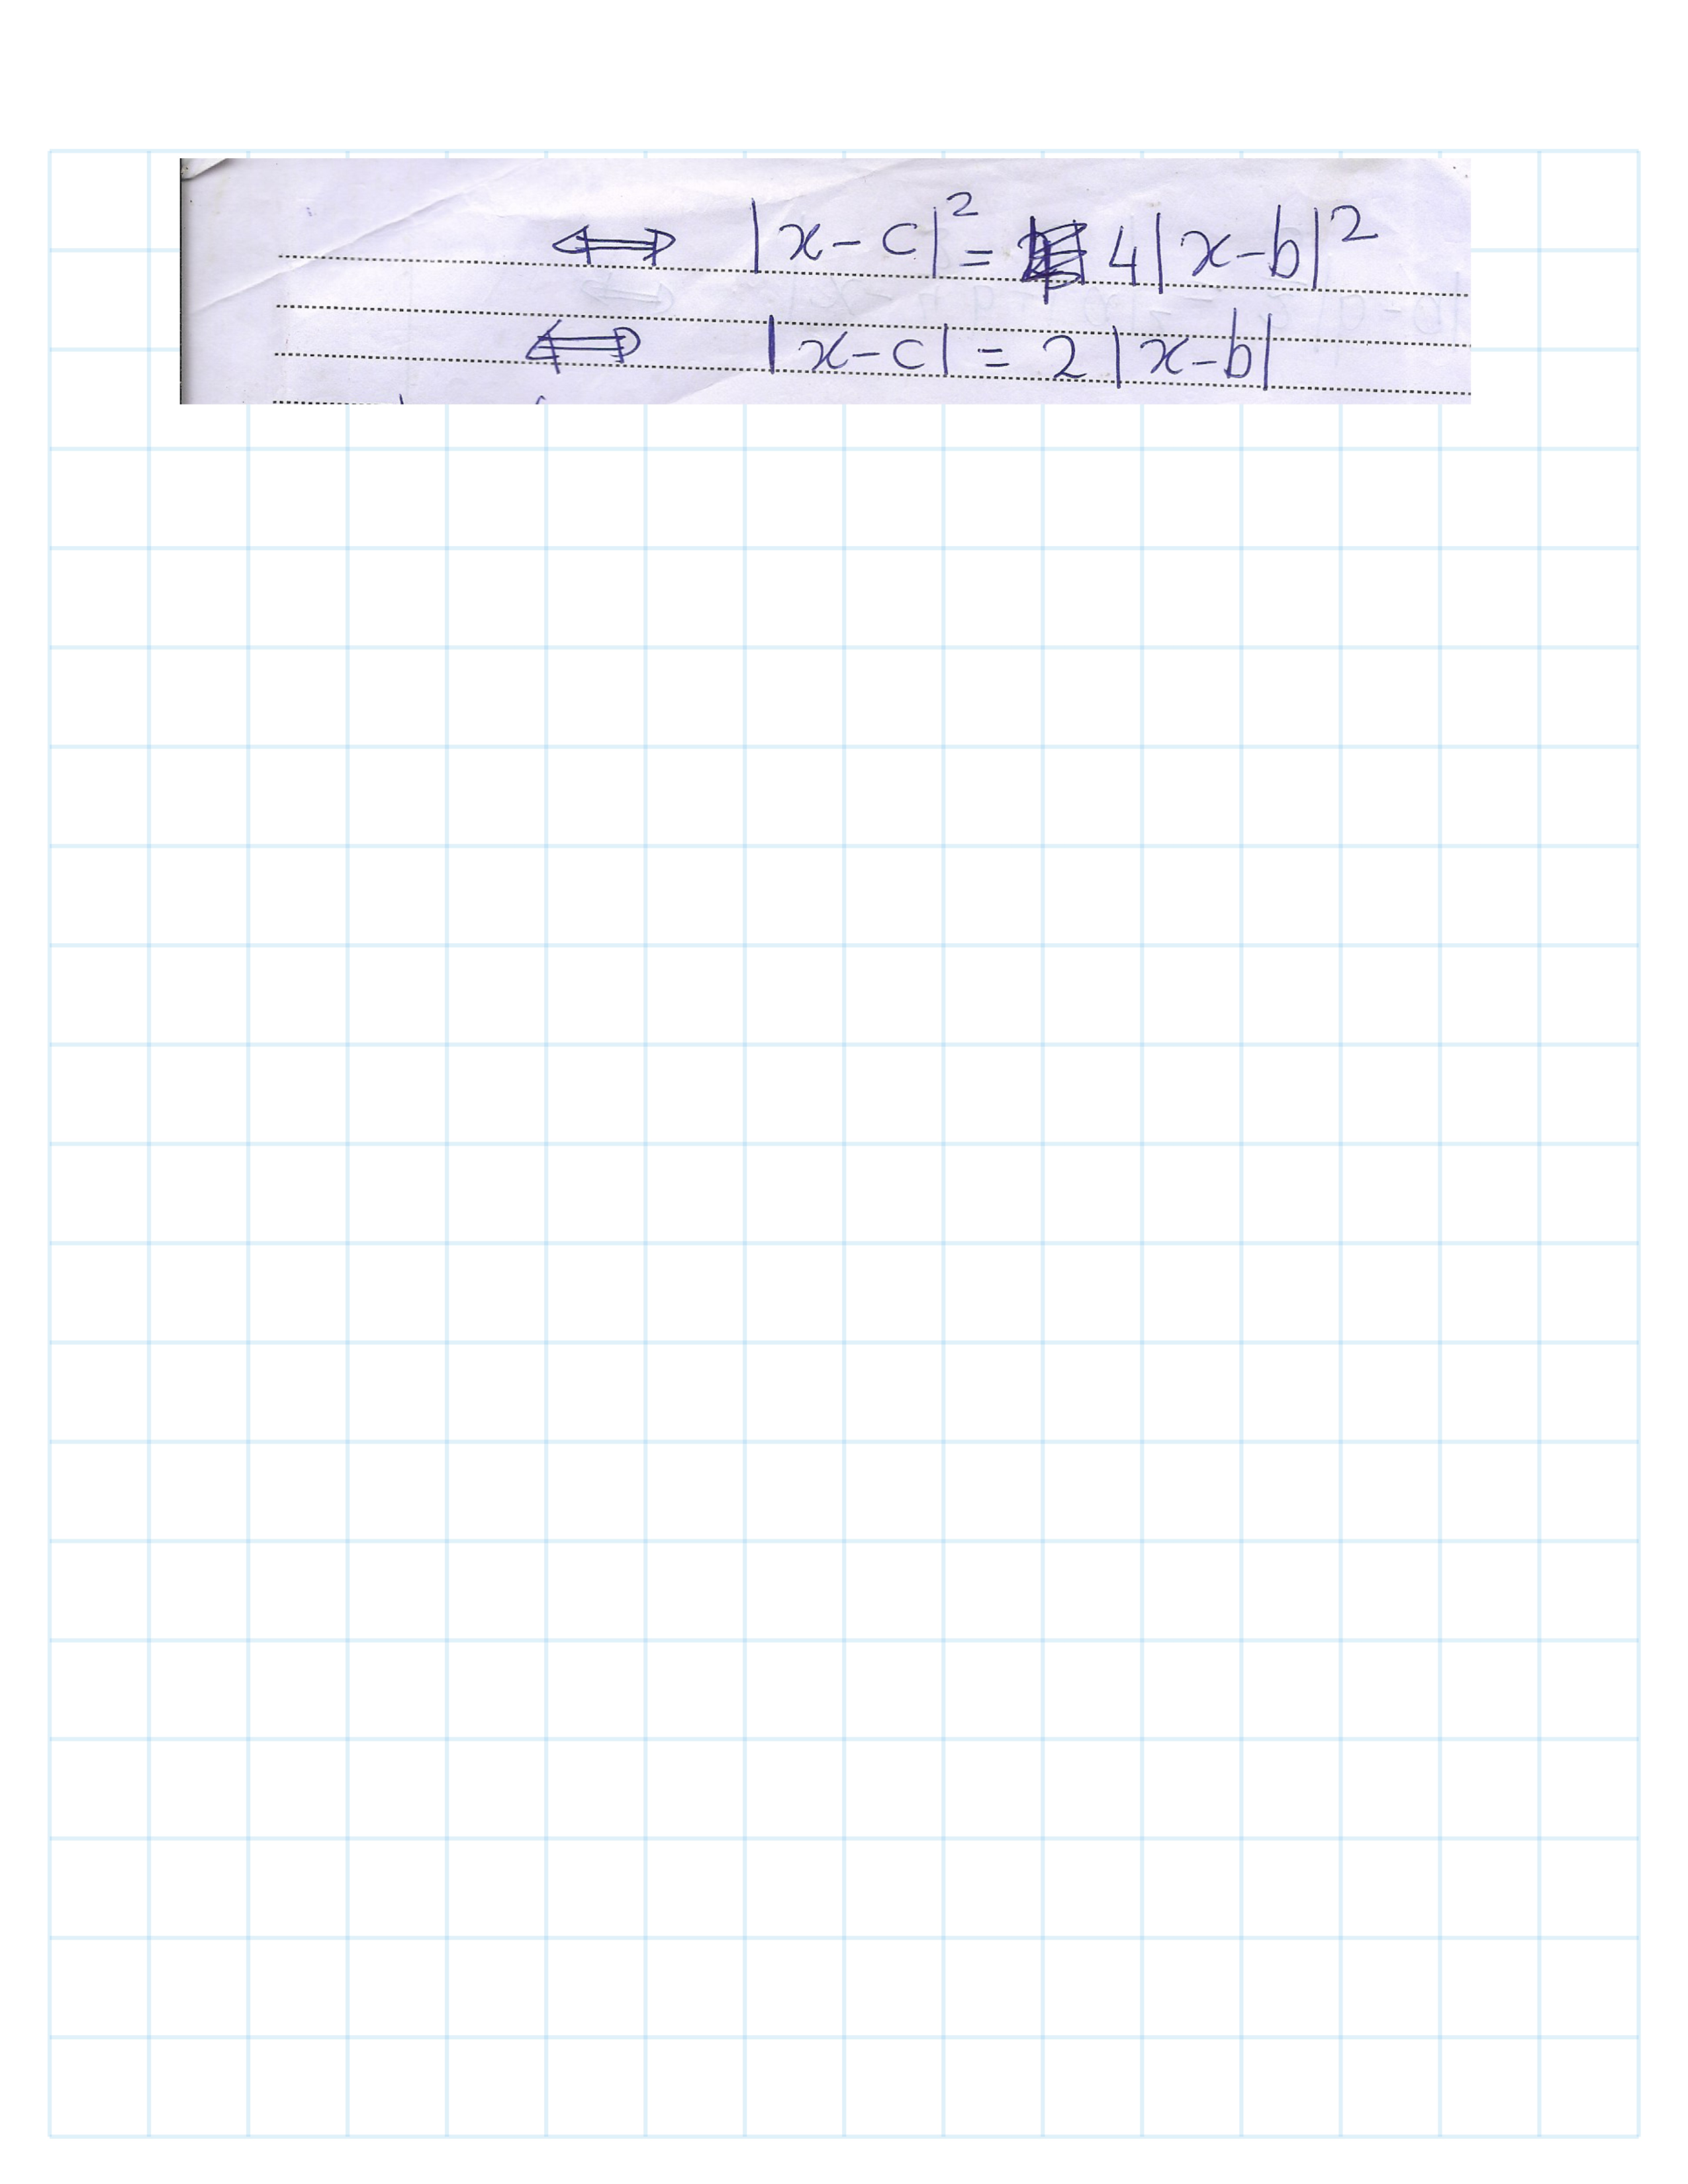
\includegraphics{Figures/Ex-1/Rudin-Ex (34).png}
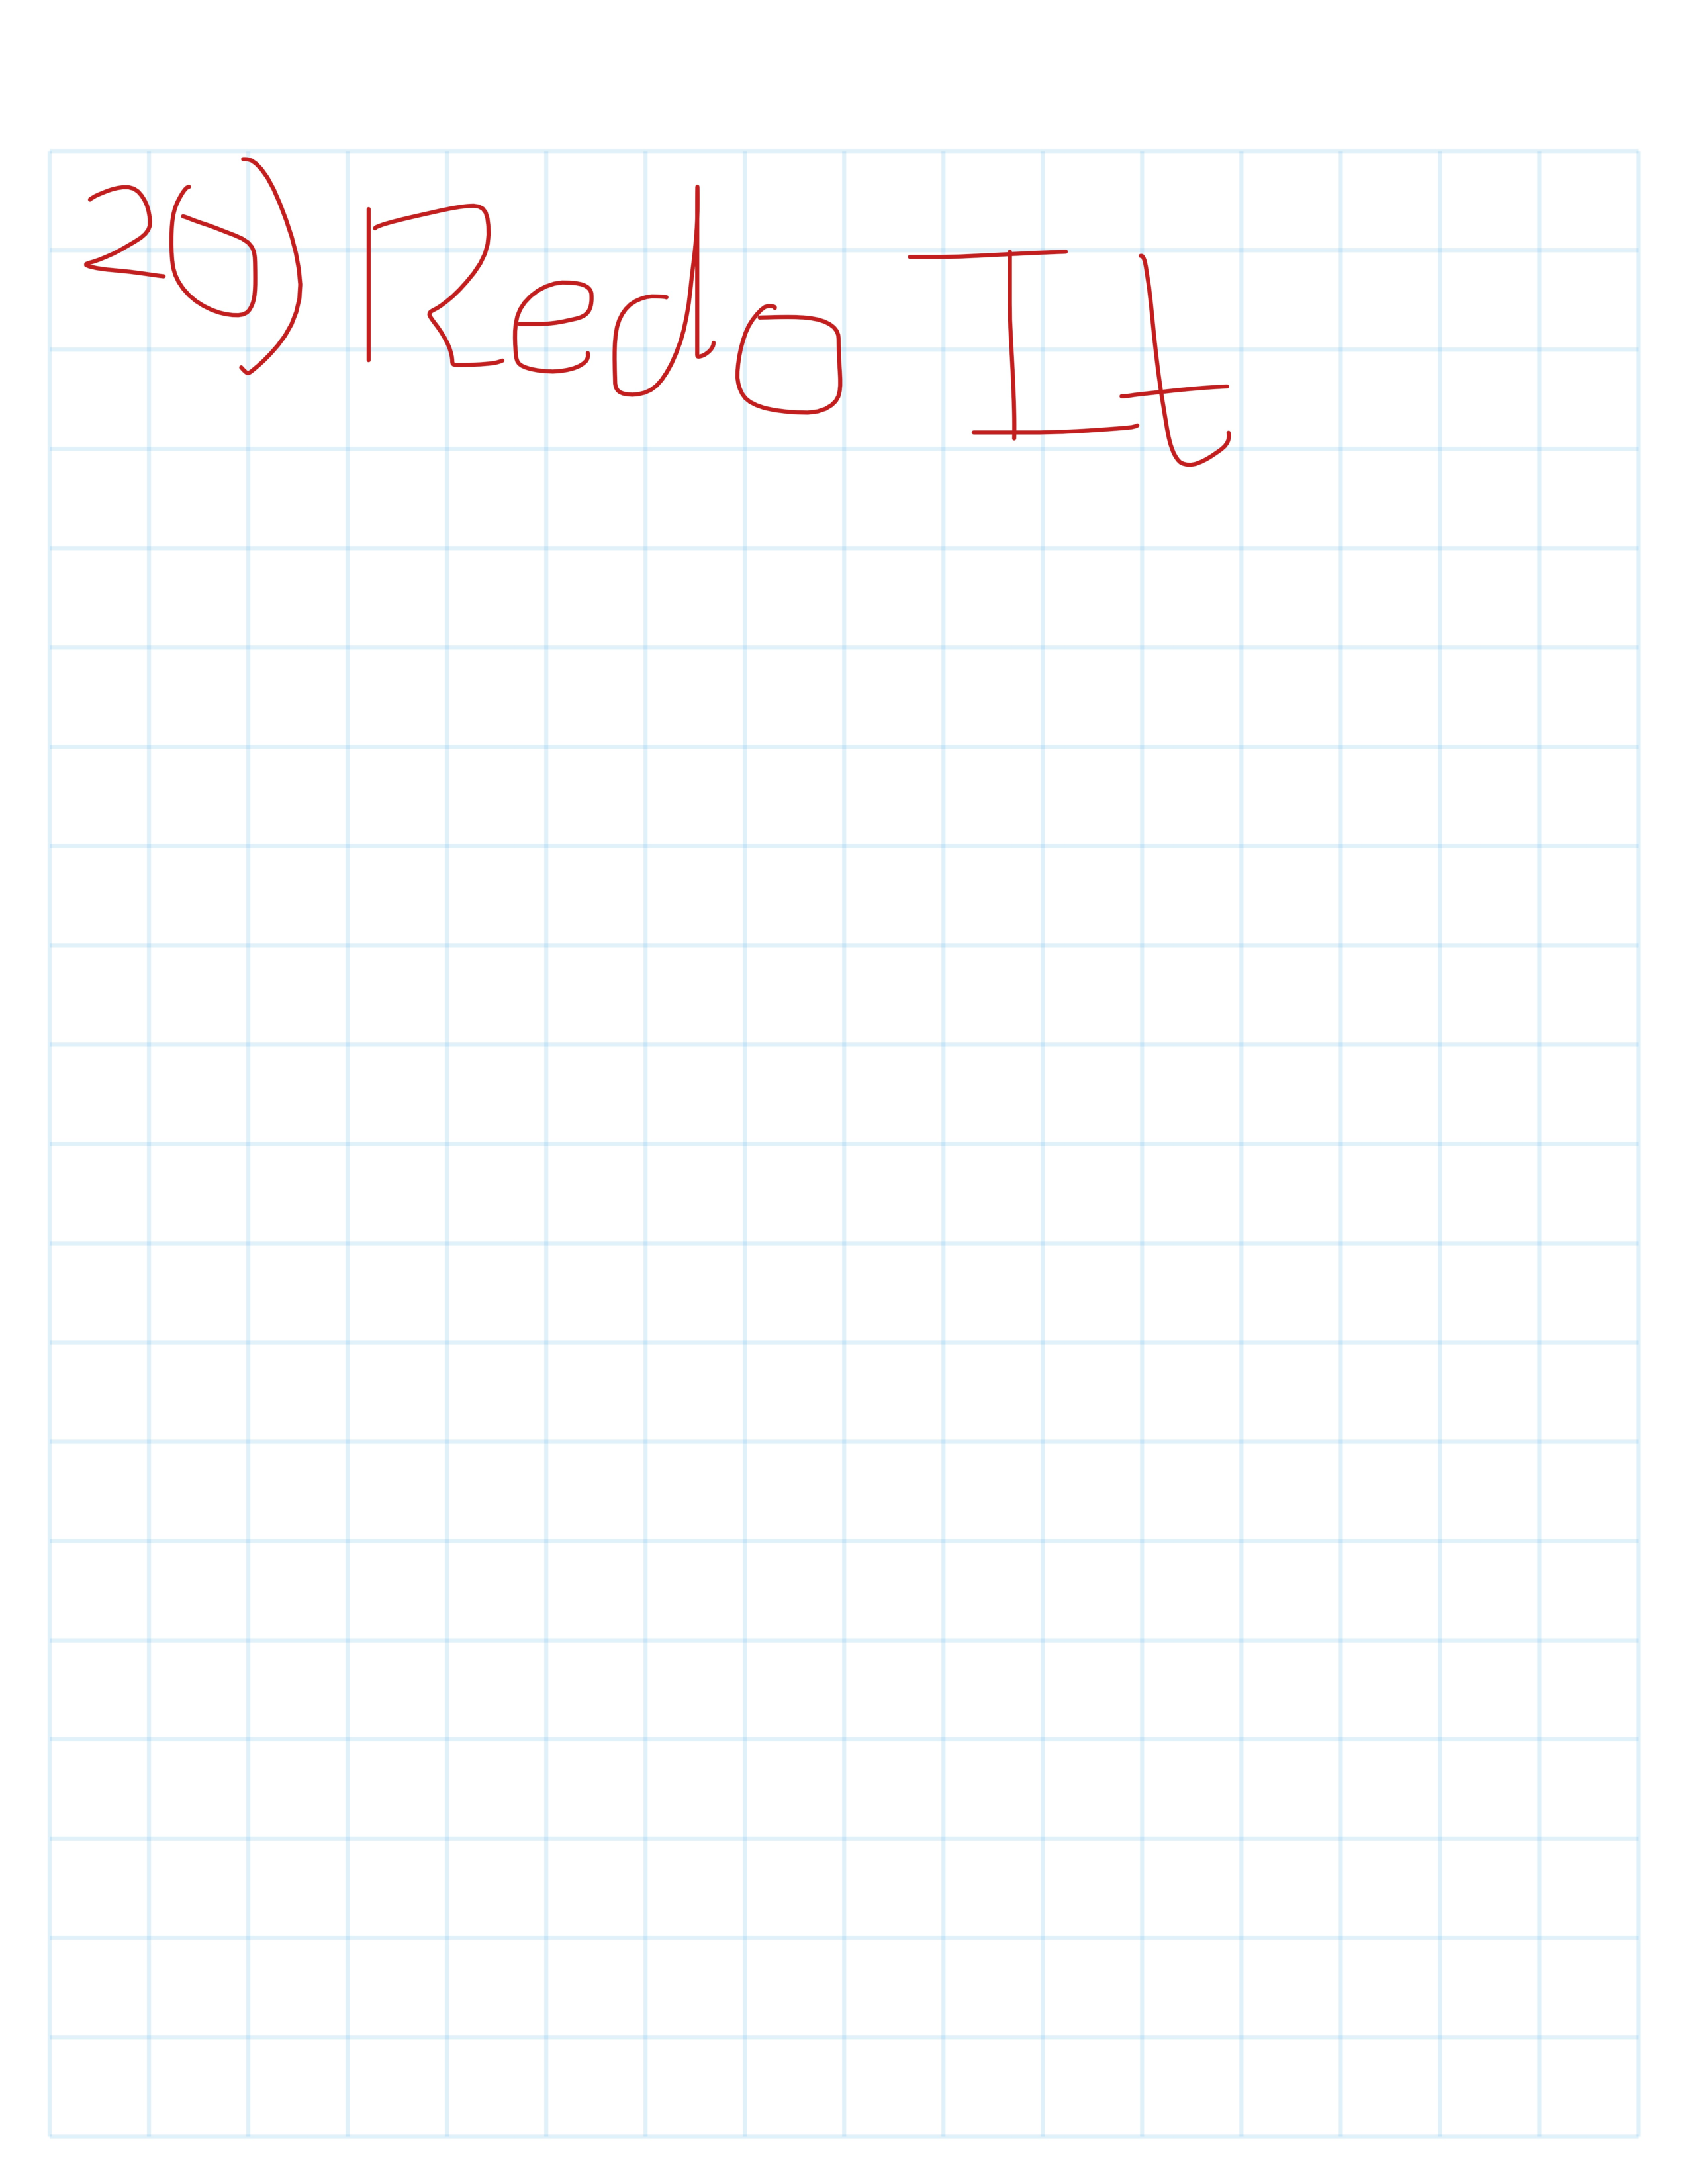
\includegraphics{Figures/Ex-1/Rudin-Ex (35).png}

\chapter{Basic Topology}\label{basic-topology}

\section{Exercise}\label{exercise-1}

\chapter{Numerical Sequences and Series}\label{numerical-sequences-and-series}

\chapter{Continuity}\label{continuity}

  \bibliography{book.bib,packages.bib}

\end{document}
